\documentclass[journal]{IEEEtran}
\usepackage[T1]{fontenc}% XeTeX (tectonic): lets IEEEtran's Times (ptm) resolve
% Journal version of paper/main.tex. Every number is a macro from ../numbers.tex (generated by
% experiments/make_macros.py from results/) or a table generated from results/. Do not type numbers.
\usepackage{graphicx,booktabs,xcolor,amsmath,amssymb,cite,url}
\usepackage{tikz}
\usetikzlibrary{positioning,arrows.meta,fit}
\def\UrlBreaks{\do\/\do\-\do\.\do\_}
\graphicspath{{../../results/}}
\newcommand{\todo}[1]{{\color{red}\textbf{[#1]}}}
% GENERATED by experiments/make_macros.py -- do not edit. Source of each macro in its trailing comment.
\newcommand{\ThreshCone}{10}% docs/SPEC.md C1 (spec constant)
\newcommand{\ThreshConeB}{100}% docs/SPEC.md C1b (spec constant)
\newcommand{\ThreshFourA}{20}% docs/SPEC.md C4a pct (spec constant)
\newcommand{\ThreshFourB}{10}% docs/SPEC.md C4b pct (spec constant)
\newcommand{\BudgetLut}{6,000}% docs/SPEC.md C3 (spec constant)
\newcommand{\BudgetMult}{40}% docs/SPEC.md C3 (spec constant)
\newcommand{\BudgetBram}{12}% docs/SPEC.md C3 (spec constant)
\newcommand{\RandomLayers}{1,000}% docs/SPEC.md C2a (spec constant)
\newcommand{\ImagesCtwoB}{10}% docs/SPEC.md C2b (spec constant)
\newcommand{\ImagesCtwoC}{100}% docs/SPEC.md C2c (spec constant)
\newcommand{\PDefault}{8}% docs/SPEC.md default P (spec constant)
\newcommand{\PMax}{16}% docs/SPEC.md P sweep (spec constant)
\newcommand{\Lanes}{4}% docs/SPEC.md DESIGN 5 lanes per output channel (spec constant)
\newcommand{\DescWords}{18}% docs/SPEC.md DESIGN 6.2 descriptor words (spec constant)
\newcommand{\WbufRows}{512}% docs/SPEC.md section 7 weight buffer rows (spec constant)
\newcommand{\PortBits}{32}% docs/SPEC.md section 2 accelerator RAM port width (spec constant)
\newcommand{\RamMiB}{1}% docs/SPEC.md section 7 simulated RAM (spec constant)
\newcommand{\Pvone}{1}% docs/SPEC.md section 2 (P grid value, table row label)
\newcommand{\Pvtwo}{2}% docs/SPEC.md section 2 (P grid value, table row label)
\newcommand{\Pvfour}{4}% docs/SPEC.md section 2 (P grid value, table row label)
\newcommand{\Pveight}{8}% docs/SPEC.md section 2 (P grid value, table row label)
\newcommand{\Pvsixteen}{16}% docs/SPEC.md section 2 (P grid value, table row label)
\newcommand{\PGrid}{1, 2, 4, 8, 16}% docs/SPEC.md section 2 (P ablation grid)
\newcommand{\MOneCommit}{6533b1e9f9f2b7c46bb8dbca5d205ab71fca11ff}% git rev-parse m1^{}
\newcommand{\MOneCommitShort}{6533b1e}% git rev-parse m1^{}
\newcommand{\MOneCsvSha}{fd94f39a1a913ee63cb03e4a9cd256cc42e6ca0df9dd0c5383c50ac62e4bd362}% sha256 of results/m1_predictions.csv at tag m1
\newcommand{\MOneCsvShaShort}{fd94f39a1a913ee6}% sha256 of results/m1_predictions.csv at tag m1
\newcommand{\MOneModelCommit}{1f4fa47}% results/m1_summary.json commit
\newcommand{\MOneRowsAll}{324}% data rows of results/m1_predictions.csv (all archs)
\newcommand{\MOneRows}{108}% rows with arch=os in results/m1_predictions.csv
\newcommand{\MOneRowsPone}{32}% rows with arch=os and P=1
\newcommand{\MOneRowsPtwo}{23}% rows with arch=os and P=2
\newcommand{\MOneRowsPfour}{19}% rows with arch=os and P=4
\newcommand{\MOneRowsPeight}{17}% rows with arch=os and P=8
\newcommand{\MOneRowsPsixteen}{17}% rows with arch=os and P=16
\newcommand{\BenchWindow}{120}% results/baseline_overhead.json cycles_median
\newcommand{\DrvChain}{71}% results/driver_overhead.json drv_chain
\newcommand{\DrvPatch}{15}% results/driver_overhead.json drv_patch
\newcommand{\BaselineCyclesMnist}{12,188,028}% results/baseline_mnist_cnn.json mcugrad_result.cycles_median
\newcommand{\BaselineMinMnist}{12,183,011}% results/baseline_mnist_cnn.json mcugrad_result.cycles_min
\newcommand{\BaselineMaxMnist}{12,193,076}% results/baseline_mnist_cnn.json mcugrad_result.cycles_max
\newcommand{\BaselineMsMnist}{243.8}% results/baseline_mnist_cnn.json cycles_median / clock_hz
\newcommand{\BaselineImagesMnist}{10}% results/baseline_mnist_cnn.json images
\newcommand{\BaselineRunsMnist}{3}% results/baseline_mnist_cnn.json runs
\newcommand{\BaselineCorrectMnist}{10}% results/baseline_mnist_cnn.json mcugrad_result.correct (of images)
\newcommand{\ClockMHzMnist}{50}% results/baseline_mnist_cnn.json clock_hz
\newcommand{\ProfileAccelShareMnist}{96.4}% sum of ops[].share with name conv2d*/matmul* in baseline_profile_mnist_cnn.json (pct)
\newcommand{\ProfileSwShareMnist}{3.6}% sum of ops[].share, pool/transpose ops, baseline_profile_mnist_cnn.json (pct)
\newcommand{\BaselineCyclesCifar}{72,157,425}% results/baseline_cifar_mobilenet.json mcugrad_result.cycles_median
\newcommand{\BaselineMinCifar}{72,132,576}% results/baseline_cifar_mobilenet.json mcugrad_result.cycles_min
\newcommand{\BaselineMaxCifar}{72,174,963}% results/baseline_cifar_mobilenet.json mcugrad_result.cycles_max
\newcommand{\BaselineMsCifar}{1443.1}% results/baseline_cifar_mobilenet.json cycles_median / clock_hz
\newcommand{\BaselineImagesCifar}{10}% results/baseline_cifar_mobilenet.json images
\newcommand{\BaselineRunsCifar}{3}% results/baseline_cifar_mobilenet.json runs
\newcommand{\BaselineCorrectCifar}{8}% results/baseline_cifar_mobilenet.json mcugrad_result.correct (of images)
\newcommand{\ClockMHzCifar}{50}% results/baseline_cifar_mobilenet.json clock_hz
\newcommand{\ProfileAccelShareCifar}{99.9}% sum of ops[].share with name conv2d*/matmul* in baseline_profile_cifar_mobilenet.json (pct)
\newcommand{\ProfileSwShareCifar}{0.1}% sum of ops[].share, pool/transpose ops, baseline_profile_cifar_mobilenet.json (pct)
\newcommand{\PredSpeedupMnistPone}{22.9}% m1_summary.json models.mnist_cnn.archs.os.P.1.predicted_speedup
\newcommand{\PredStampMnistPone}{98,312}% m1_summary.json models.mnist_cnn.archs.os.P.1.sum_stamp
\newcommand{\PredModelRunMnistPone}{531,982}% m1_summary.json models.mnist_cnn.archs.os.P.1.predicted_model_run
\newcommand{\PredSpeedupMnistPtwo}{25.2}% m1_summary.json models.mnist_cnn.archs.os.P.2.predicted_speedup
\newcommand{\PredStampMnistPtwo}{50,888}% m1_summary.json models.mnist_cnn.archs.os.P.2.sum_stamp
\newcommand{\PredModelRunMnistPtwo}{484,524}% m1_summary.json models.mnist_cnn.archs.os.P.2.predicted_model_run
\newcommand{\PredSpeedupMnistPfour}{26.4}% m1_summary.json models.mnist_cnn.archs.os.P.4.predicted_speedup
\newcommand{\PredStampMnistPfour}{27,697}% m1_summary.json models.mnist_cnn.archs.os.P.4.sum_stamp
\newcommand{\PredModelRunMnistPfour}{461,316}% m1_summary.json models.mnist_cnn.archs.os.P.4.predicted_model_run
\newcommand{\PredSpeedupMnistPeight}{27.0}% m1_summary.json models.mnist_cnn.archs.os.P.8.predicted_speedup
\newcommand{\PredStampMnistPeight}{18,496}% m1_summary.json models.mnist_cnn.archs.os.P.8.sum_stamp
\newcommand{\PredModelRunMnistPeight}{452,098}% m1_summary.json models.mnist_cnn.archs.os.P.8.predicted_model_run
\newcommand{\PredSpeedupMnistPsixteen}{27.2}% m1_summary.json models.mnist_cnn.archs.os.P.16.predicted_speedup
\newcommand{\PredStampMnistPsixteen}{15,156}% m1_summary.json models.mnist_cnn.archs.os.P.16.sum_stamp
\newcommand{\PredModelRunMnistPsixteen}{448,758}% m1_summary.json models.mnist_cnn.archs.os.P.16.predicted_model_run
\newcommand{\PredAccelChainsMnistPeight}{18,508}% m1_summary.json models.mnist_cnn.archs.os.P.8.accel_cycles
\newcommand{\PredSwCyclesMnistPeight}{433,242}% m1_summary.json models.mnist_cnn.archs.os.P.8.sw_cycles
\newcommand{\PredDriverMnistPeight}{228}% m1_summary.json models.mnist_cnn.archs.os.P.8.driver_cycles
\newcommand{\PredCfourBMnistPeight}{18,736}% m1_summary.json models.mnist_cnn.archs.os.P.8.c4b_pred_cycles
\newcommand{\PredCommandsMnistPeight}{3}% m1_summary.json models.mnist_cnn.archs.os.P.8.n_commands
\newcommand{\PredChainsMnistPeight}{3}% m1_summary.json models.mnist_cnn.archs.os.P.8.n_chains
\newcommand{\PredUtilMnistPeight}{56.1}% m1_summary.json models.mnist_cnn.archs.os.P.8.util (pct)
\newcommand{\PredSwShareMnistPeight}{95.8}% m1_summary.json models.mnist_cnn.archs.os.P.8.sw_cycles / predicted_model_run (pct)
\newcommand{\PredPstarMnist}{16}% m1_summary.json models.mnist_cnn.archs.os.p_star (16 = not reached)
\newcommand{\PredPstarEndMnist}{2}% m1_summary.json models.mnist_cnn.archs.os.p_star_end_to_end
\newcommand{\PredSpeedupCifarPone}{111.7}% m1_summary.json models.cifar_mobilenet.archs.os.P.1.predicted_speedup
\newcommand{\PredStampCifarPone}{582,676}% m1_summary.json models.cifar_mobilenet.archs.os.P.1.sum_stamp
\newcommand{\PredModelRunCifarPone}{645,778}% m1_summary.json models.cifar_mobilenet.archs.os.P.1.predicted_model_run
\newcommand{\PredSpeedupCifarPtwo}{187.1}% m1_summary.json models.cifar_mobilenet.archs.os.P.2.predicted_speedup
\newcommand{\PredStampCifarPtwo}{322,660}% m1_summary.json models.cifar_mobilenet.archs.os.P.2.sum_stamp
\newcommand{\PredModelRunCifarPtwo}{385,748}% m1_summary.json models.cifar_mobilenet.archs.os.P.2.predicted_model_run
\newcommand{\PredSpeedupCifarPfour}{282.0}% m1_summary.json models.cifar_mobilenet.archs.os.P.4.predicted_speedup
\newcommand{\PredStampCifarPfour}{192,788}% m1_summary.json models.cifar_mobilenet.archs.os.P.4.sum_stamp
\newcommand{\PredModelRunCifarPfour}{255,870}% m1_summary.json models.cifar_mobilenet.archs.os.P.4.predicted_model_run
\newcommand{\PredSpeedupCifarPeight}{363.1}% m1_summary.json models.cifar_mobilenet.archs.os.P.8.predicted_speedup
\newcommand{\PredStampCifarPeight}{135,672}% m1_summary.json models.cifar_mobilenet.archs.os.P.8.sum_stamp
\newcommand{\PredModelRunCifarPeight}{198,752}% m1_summary.json models.cifar_mobilenet.archs.os.P.8.predicted_model_run
\newcommand{\PredSpeedupCifarPsixteen}{411.4}% m1_summary.json models.cifar_mobilenet.archs.os.P.16.predicted_speedup
\newcommand{\PredStampCifarPsixteen}{112,308}% m1_summary.json models.cifar_mobilenet.archs.os.P.16.sum_stamp
\newcommand{\PredModelRunCifarPsixteen}{175,388}% m1_summary.json models.cifar_mobilenet.archs.os.P.16.predicted_model_run
\newcommand{\PredAccelChainsCifarPeight}{135,704}% m1_summary.json models.cifar_mobilenet.archs.os.P.8.accel_cycles
\newcommand{\PredSwCyclesCifarPeight}{62,756}% m1_summary.json models.cifar_mobilenet.archs.os.P.8.sw_cycles
\newcommand{\PredDriverCifarPeight}{172}% m1_summary.json models.cifar_mobilenet.archs.os.P.8.driver_cycles
\newcommand{\PredCfourBCifarPeight}{135,876}% m1_summary.json models.cifar_mobilenet.archs.os.P.8.c4b_pred_cycles
\newcommand{\PredCommandsCifarPeight}{14}% m1_summary.json models.cifar_mobilenet.archs.os.P.8.n_commands
\newcommand{\PredChainsCifarPeight}{2}% m1_summary.json models.cifar_mobilenet.archs.os.P.8.n_chains
\newcommand{\PredUtilCifarPeight}{45.0}% m1_summary.json models.cifar_mobilenet.archs.os.P.8.util (pct)
\newcommand{\PredSwShareCifarPeight}{31.6}% m1_summary.json models.cifar_mobilenet.archs.os.P.8.sw_cycles / predicted_model_run (pct)
\newcommand{\PredPstarCifar}{16}% m1_summary.json models.cifar_mobilenet.archs.os.p_star (16 = not reached)
\newcommand{\PredPstarEndCifar}{16}% m1_summary.json models.cifar_mobilenet.archs.os.p_star_end_to_end
\newcommand{\MeasCyclesMnistPone}{\todo{MEASURE: accelerated cycles mnist cnn P=1}}% PENDING results/m5_accel_mnist_cnn_P1.json
\newcommand{\MeasSpeedupMnistPone}{\todo{MEASURE: speedup mnist cnn P=1}}% PENDING results/m5_accel_mnist_cnn_P1.json
\newcommand{\MeasCyclesMnistPtwo}{\todo{MEASURE: accelerated cycles mnist cnn P=2}}% PENDING results/m5_accel_mnist_cnn_P2.json
\newcommand{\MeasSpeedupMnistPtwo}{\todo{MEASURE: speedup mnist cnn P=2}}% PENDING results/m5_accel_mnist_cnn_P2.json
\newcommand{\MeasCyclesMnistPfour}{\todo{MEASURE: accelerated cycles mnist cnn P=4}}% PENDING results/m5_accel_mnist_cnn_P4.json
\newcommand{\MeasSpeedupMnistPfour}{\todo{MEASURE: speedup mnist cnn P=4}}% PENDING results/m5_accel_mnist_cnn_P4.json
\newcommand{\MeasCyclesMnistPeight}{\todo{MEASURE: accelerated cycles mnist cnn P=8}}% PENDING results/m5_accel_mnist_cnn_P8.json
\newcommand{\MeasSpeedupMnistPeight}{\todo{MEASURE: speedup mnist cnn P=8}}% PENDING results/m5_accel_mnist_cnn_P8.json
\newcommand{\MeasCyclesMnistPsixteen}{\todo{MEASURE: accelerated cycles mnist cnn P=16}}% PENDING results/m5_accel_mnist_cnn_P16.json
\newcommand{\MeasSpeedupMnistPsixteen}{\todo{MEASURE: speedup mnist cnn P=16}}% PENDING results/m5_accel_mnist_cnn_P16.json
\newcommand{\MeasCyclesCifarPone}{\todo{MEASURE: accelerated cycles cifar mobilenet P=1}}% PENDING results/m5_accel_cifar_mobilenet_P1.json
\newcommand{\MeasSpeedupCifarPone}{\todo{MEASURE: speedup cifar mobilenet P=1}}% PENDING results/m5_accel_cifar_mobilenet_P1.json
\newcommand{\MeasCyclesCifarPtwo}{\todo{MEASURE: accelerated cycles cifar mobilenet P=2}}% PENDING results/m5_accel_cifar_mobilenet_P2.json
\newcommand{\MeasSpeedupCifarPtwo}{\todo{MEASURE: speedup cifar mobilenet P=2}}% PENDING results/m5_accel_cifar_mobilenet_P2.json
\newcommand{\MeasCyclesCifarPfour}{\todo{MEASURE: accelerated cycles cifar mobilenet P=4}}% PENDING results/m5_accel_cifar_mobilenet_P4.json
\newcommand{\MeasSpeedupCifarPfour}{\todo{MEASURE: speedup cifar mobilenet P=4}}% PENDING results/m5_accel_cifar_mobilenet_P4.json
\newcommand{\MeasCyclesCifarPeight}{\todo{MEASURE: accelerated cycles cifar mobilenet P=8}}% PENDING results/m5_accel_cifar_mobilenet_P8.json
\newcommand{\MeasSpeedupCifarPeight}{\todo{MEASURE: speedup cifar mobilenet P=8}}% PENDING results/m5_accel_cifar_mobilenet_P8.json
\newcommand{\MeasCyclesCifarPsixteen}{\todo{MEASURE: accelerated cycles cifar mobilenet P=16}}% PENDING results/m5_accel_cifar_mobilenet_P16.json
\newcommand{\MeasSpeedupCifarPsixteen}{\todo{MEASURE: speedup cifar mobilenet P=16}}% PENDING results/m5_accel_cifar_mobilenet_P16.json
\newcommand{\VerdictCone}{\todo{MEASURE: C1 verdict}}% PENDING C1 from m5_accel_*_P8.json
\newcommand{\VerdictConeB}{\todo{MEASURE: C1b verdict}}% PENDING C1b from m5_accel_cifar_mobilenet_P8.json
\newcommand{\MeasCtwoALayers}{\todo{MEASURE: C2a layers run}}% PENDING results/m3_bitexact.csv
\newcommand{\MeasCtwoAMismatch}{\todo{MEASURE: C2a mismatching bytes}}% PENDING results/m3_bitexact.csv
\newcommand{\VerdictCtwoA}{\todo{MEASURE: C2a verdict}}% PENDING results/m3_bitexact.csv
\newcommand{\MeasCtwoBImages}{\todo{MEASURE: c2b images}}% PENDING results/m5_bitexact.json
\newcommand{\MeasCtwoBMismatch}{\todo{MEASURE: c2b mismatch}}% PENDING results/m5_bitexact.json
\newcommand{\MeasCtwoCImages}{\todo{MEASURE: c2c images}}% PENDING results/m5_bitexact.json
\newcommand{\MeasCtwoCMismatch}{\todo{MEASURE: c2c mismatch}}% PENDING results/m5_bitexact.json
\newcommand{\SynPicorvLut}{2,896}% results/syn/picorv32.jsonl seed 1 .lut4
\newcommand{\SynPicorvFf}{1,027}% results/syn/picorv32.jsonl seed 1 .ff
\newcommand{\SynPicorvBram}{0}% results/syn/picorv32.jsonl seed 1 .dp16kd
\newcommand{\SynPicorvMult}{4}% results/syn/picorv32.jsonl seed 1 .mult18x18d
\newcommand{\SynPicorvFmax}{78.2}% results/syn/picorv32.jsonl median fmax_mhz over 1 seeds
\newcommand{\SynPicorvFmaxSeeds}{1}% results/syn/picorv32.jsonl seeds
\newcommand{\SynSocNoAccelLut}{3,224}% results/syn/soc_noaccel.jsonl seed 1 .lut4
\newcommand{\SynSocNoAccelFf}{1,073}% results/syn/soc_noaccel.jsonl seed 1 .ff
\newcommand{\SynSocNoAccelBram}{128}% results/syn/soc_noaccel.jsonl seed 1 .dp16kd
\newcommand{\SynSocNoAccelMult}{4}% results/syn/soc_noaccel.jsonl seed 1 .mult18x18d
\newcommand{\SynSocNoAccelFmax}{63.1}% results/syn/soc_noaccel.jsonl median fmax_mhz over 1 seeds
\newcommand{\SynSocNoAccelFmaxSeeds}{1}% results/syn/soc_noaccel.jsonl seeds
\newcommand{\SynSocPeightLut}{\todo{MEASURE: soc lut4}}% PENDING results/syn/soc_P8.jsonl
\newcommand{\SynSocPeightFf}{\todo{MEASURE: soc ff}}% PENDING results/syn/soc_P8.jsonl
\newcommand{\SynSocPeightBram}{\todo{MEASURE: soc dp16kd}}% PENDING results/syn/soc_P8.jsonl
\newcommand{\SynSocPeightMult}{\todo{MEASURE: soc mult18x18d}}% PENDING results/syn/soc_P8.jsonl
\newcommand{\SynSocPeightFmax}{\todo{MEASURE: soc Fmax}}% PENDING results/syn/soc_P8.jsonl
\newcommand{\SynSocPeightFmaxSeeds}{\todo{MEASURE: soc seeds}}% PENDING results/syn/soc_P8.jsonl
\newcommand{\SynAccelPoneLut}{\todo{MEASURE: accel lut4}}% PENDING results/syn/accel_P1.jsonl
\newcommand{\SynAccelPoneFf}{\todo{MEASURE: accel ff}}% PENDING results/syn/accel_P1.jsonl
\newcommand{\SynAccelPoneBram}{\todo{MEASURE: accel dp16kd}}% PENDING results/syn/accel_P1.jsonl
\newcommand{\SynAccelPoneMult}{\todo{MEASURE: accel mult18x18d}}% PENDING results/syn/accel_P1.jsonl
\newcommand{\SynAccelPoneFmax}{\todo{MEASURE: accel Fmax}}% PENDING results/syn/accel_P1.jsonl
\newcommand{\SynAccelPoneFmaxSeeds}{\todo{MEASURE: accel seeds}}% PENDING results/syn/accel_P1.jsonl
\newcommand{\SynAccelPtwoLut}{\todo{MEASURE: accel lut4}}% PENDING results/syn/accel_P2.jsonl
\newcommand{\SynAccelPtwoFf}{\todo{MEASURE: accel ff}}% PENDING results/syn/accel_P2.jsonl
\newcommand{\SynAccelPtwoBram}{\todo{MEASURE: accel dp16kd}}% PENDING results/syn/accel_P2.jsonl
\newcommand{\SynAccelPtwoMult}{\todo{MEASURE: accel mult18x18d}}% PENDING results/syn/accel_P2.jsonl
\newcommand{\SynAccelPtwoFmax}{\todo{MEASURE: accel Fmax}}% PENDING results/syn/accel_P2.jsonl
\newcommand{\SynAccelPtwoFmaxSeeds}{\todo{MEASURE: accel seeds}}% PENDING results/syn/accel_P2.jsonl
\newcommand{\SynAccelPfourLut}{\todo{MEASURE: accel lut4}}% PENDING results/syn/accel_P4.jsonl
\newcommand{\SynAccelPfourFf}{\todo{MEASURE: accel ff}}% PENDING results/syn/accel_P4.jsonl
\newcommand{\SynAccelPfourBram}{\todo{MEASURE: accel dp16kd}}% PENDING results/syn/accel_P4.jsonl
\newcommand{\SynAccelPfourMult}{\todo{MEASURE: accel mult18x18d}}% PENDING results/syn/accel_P4.jsonl
\newcommand{\SynAccelPfourFmax}{\todo{MEASURE: accel Fmax}}% PENDING results/syn/accel_P4.jsonl
\newcommand{\SynAccelPfourFmaxSeeds}{\todo{MEASURE: accel seeds}}% PENDING results/syn/accel_P4.jsonl
\newcommand{\SynAccelPeightLut}{\todo{MEASURE: accel lut4}}% PENDING results/syn/accel_P8.jsonl
\newcommand{\SynAccelPeightFf}{\todo{MEASURE: accel ff}}% PENDING results/syn/accel_P8.jsonl
\newcommand{\SynAccelPeightBram}{\todo{MEASURE: accel dp16kd}}% PENDING results/syn/accel_P8.jsonl
\newcommand{\SynAccelPeightMult}{\todo{MEASURE: accel mult18x18d}}% PENDING results/syn/accel_P8.jsonl
\newcommand{\SynAccelPeightFmax}{\todo{MEASURE: accel Fmax}}% PENDING results/syn/accel_P8.jsonl
\newcommand{\SynAccelPeightFmaxSeeds}{\todo{MEASURE: accel seeds}}% PENDING results/syn/accel_P8.jsonl
\newcommand{\SynAccelPsixteenLut}{\todo{MEASURE: accel lut4}}% PENDING results/syn/accel_P16.jsonl
\newcommand{\SynAccelPsixteenFf}{\todo{MEASURE: accel ff}}% PENDING results/syn/accel_P16.jsonl
\newcommand{\SynAccelPsixteenBram}{\todo{MEASURE: accel dp16kd}}% PENDING results/syn/accel_P16.jsonl
\newcommand{\SynAccelPsixteenMult}{\todo{MEASURE: accel mult18x18d}}% PENDING results/syn/accel_P16.jsonl
\newcommand{\SynAccelPsixteenFmax}{\todo{MEASURE: accel Fmax}}% PENDING results/syn/accel_P16.jsonl
\newcommand{\SynAccelPsixteenFmaxSeeds}{\todo{MEASURE: accel seeds}}% PENDING results/syn/accel_P16.jsonl
\newcommand{\VerdictCthree}{\todo{MEASURE: C3 verdict}}% PENDING C3 from syn/accel_P8.jsonl
\newcommand{\MeasCfourRows}{\todo{MEASURE: C4a rows}}% PENDING results/m6_pred_vs_meas.csv
\newcommand{\MeasCfourMaxErr}{\todo{MEASURE: C4a max error}}% PENDING results/m6_pred_vs_meas.csv
\newcommand{\MeasCfourMedianErr}{\todo{MEASURE: C4a median signed error}}% PENDING results/m6_pred_vs_meas.csv
\newcommand{\MeasCfourViolations}{\todo{MEASURE: C4a violations}}% PENDING results/m6_pred_vs_meas.csv
\newcommand{\VerdictCfourA}{\todo{MEASURE: C4a verdict}}% PENDING results/m6_pred_vs_meas.csv
\newcommand{\MeasCfourBMnist}{\todo{MEASURE: C4b measured mnist cnn}}% PENDING results/m6_c4b.json
\newcommand{\MeasCfourBErrMnist}{\todo{MEASURE: C4b error mnist cnn}}% PENDING results/m6_c4b.json
\newcommand{\MeasCfourBCifar}{\todo{MEASURE: C4b measured cifar mobilenet}}% PENDING results/m6_c4b.json
\newcommand{\MeasCfourBErrCifar}{\todo{MEASURE: C4b error cifar mobilenet}}% PENDING results/m6_c4b.json
\newcommand{\PstarMeasMnist}{\todo{MEASURE: measured saturation width}}% PENDING results/m5_accel_*_P*.json (sum STAMP)
\newcommand{\PstarMeasCifar}{\todo{MEASURE: measured saturation width}}% PENDING results/m5_accel_*_P*.json (sum STAMP)

\newcommand{\tabtodo}{\renewcommand{\todo}[1]{{\color{red}\textbf{?}}}}% compact pending marker inside tables
\newcommand{\sys}{\textsc{mcuaccel}}
\newcommand{\row}[1]{\csname Pv#1\endcsname & \csname PredSpeedupMnistP#1\endcsname & \csname MeasSpeedupMnistP#1\endcsname & \csname PredSpeedupCifarP#1\endcsname & \csname MeasSpeedupCifarP#1\endcsname\\}
\newcommand{\crow}[1]{\csname Pv#1\endcsname & \csname MOneRowsP#1\endcsname & \csname CfourMaxErrP#1\endcsname & \csname CfourMedErrP#1\endcsname\\}
\newcommand{\srow}[1]{\csname Pv#1\endcsname & \csname PredStampMnistP#1\endcsname & \csname MeasStampMnistP#1\endcsname & \csname PredStampCifarP#1\endcsname & \csname MeasStampCifarP#1\endcsname\\}
\newcommand{\synrow}[2]{#1 & \csname Syn#2Lut\endcsname & \csname Syn#2Ff\endcsname & \csname Syn#2Mult\endcsname & \csname Syn#2Bram\endcsname & \csname Syn#2Fmax\endcsname & \csname Syn#2FmaxSeeds\endcsname\\}
\newcommand{\code}[1]{\texttt{#1}}

\begin{document}
\title{Scoring a Frozen Cycle Model: A Small Bit-Exact int8 CNN Accelerator for a RISC-V Microcontroller SoC, Its Compiler Backend, and a Pre-Registered Evaluation}
\author{Anirudh~Sahu%
\thanks{A. Sahu is an independent researcher (e-mail: anirudh12sahu@gmail.com).}}
\markboth{Journal version, draft}{Sahu: Scoring a Frozen Cycle Model for a Small int8 CNN Accelerator}
\maketitle

\begin{abstract}
We present \sys{}, a from-scratch int8 convolution, depthwise and fully connected accelerator memory-mapped into a PicoRV32 system-on-chip, together with a backend for the \texttt{mcugrad} compiler that emits chained command descriptors and driver C while every other operator stays in the compiler's own software kernels. The accelerator is bit-exact with the TFLite/gemmlowp integer reference. The evaluation is organised as a pre-registration: five claims with fixed thresholds, and an analytic port-bound cycle model of the accelerator, its driver and the fallback operators, were committed to git (tag \texttt{m1}, \MOneCommitShort) before any datapath or sequencer RTL existed, and the RTL was then scored against the frozen predictions. We give the full architecture, every equation of the model, the backend, the verification campaign and the scored outcome. Over \MOneRows{} accelerator commands at five array widths ($P\in\{\PGrid\}$) the frozen model predicts every command within \MeasCfourMaxErr\,\% (median signed error \MeasCfourMedianErr\,\%) and each network's accelerator-plus-driver time within \MeasCfourBErrMnist\,\% and \MeasCfourBErrCifar\,\%; \NExceed{} scored (command, width) rows exceed their pre-registered bias, and for all \TieNProbed{} an RTL probe identifies the mechanism after the fact: writes granted during the pixel setup cycle that the model charges serially. At $P=\PDefault$ the measured end-to-end cycle speedups over the same small, non-pipelined core are \MeasSpeedupMnistPeight$\times$ (\texttt{mnist\_cnn}) and \MeasSpeedupCifarPeight$\times$ (\texttt{cifar\_mobilenet}); \MeasCtwoALayers{} random layers and whole-network runs show zero mismatching bytes. The LUT budget is refuted: \SynAccelPeightLut{} LUT4 against \BudgetLut{}. All cycle counts are cycle-accurate RTL simulation, not board wall-clock; in our ECP5 flow the integrated SoC closes timing at \SynSocPeightFmax{}\,MHz with the accelerator and \SynSocNoAccelFmax{}\,MHz without it, a factor any wall-clock speedup must absorb.
\end{abstract}

\begin{IEEEkeywords}
Hardware accelerators, convolutional neural networks, integer quantization, RISC-V, performance modeling, pre-registration, FPGA, bit-exact verification.
\end{IEEEkeywords}

\section{Introduction}\label{sec:intro}
\IEEEPARstart{Q}{uantized} convolutional networks cost tens of millions of cycles per image on a microcontroller-class core: on the scalar RV32IM core of this study, the two networks we evaluate take \BaselineCyclesMnist{} and \BaselineCyclesCifar{} cycles per inference in software. That a dedicated int8 accelerator beats such a core by an order of magnitude or more is well established~\cite{genc2021gemmini,prakash2023cfu,moreau2018vta,yildirim2025dsc}, and reproducing that effect is not our contribution. We ask two narrower questions. First, how well does a simple analytic cycle model, written down \emph{before} the hardware exists, predict the cycle counts of a small memory-bound accelerator, with error tolerances fixed in advance? Second, when the accelerated operators are fast, which parts of a whole-network inference remain, and how do they change with the width of the multiply-accumulate array?

Analytic models of accelerators are common~\cite{zhang2015optimizing,alwani2016fused,williams2009roofline}, but they are usually developed alongside the design they describe, so their reported agreement includes whatever adjustment happened during development. We borrow the practice of pre-registration from the empirical sciences: the claims, their thresholds and the model's predictions were committed to version control before any datapath or sequencer register-transfer-level (RTL) code, with a written list of the model's known biases, and the RTL was scored at its first full measurement. Deviations found afterwards are logged and explained, not absorbed. We found no prior accelerator evaluation that froze its cycle model and error tolerances before the RTL existed (Sec.~\ref{sec:related}); the model itself is not claimed as novel, and the freeze is only as credible as the git history that records it (Sec.~\ref{sec:threats}).

\subsection{Pre-registered claims}
The claims below are quoted in substance from \texttt{docs/SPEC.md}; the predictions are frozen at tag \texttt{m1} (commit \texttt{\MOneCommitShort}, \texttt{m1\_predictions.csv} sha256 prefix \texttt{\MOneCsvShaShort}).
\begin{description}\setlength{\itemsep}{1pt}
\item[C1] The end-to-end speedup at $P=\PDefault$ output channels per tile is at least \ThreshCone$\times$ on both networks, with fallback layers and driver included. \textbf{C1b}: at least \ThreshConeB$\times$ on \texttt{cifar\_mobilenet}.
\item[C2] Bit-exactness: zero mismatching output bytes on \RandomLayers{} random layers (C2a), in every intermediate tensor of both networks for \ImagesCtwoB{} images (C2b), and in the final outputs of \ImagesCtwoC{} images per network on the full SoC, against the integer simulator and against the software baseline's outputs (C2c).
\item[C3] At $P=\PDefault$ the accelerator uses at most \BudgetLut{} LUT4, \BudgetMult{} \texttt{MULT18X18D} and \BudgetBram{} \texttt{DP16KD} on a Lattice ECP5 LFE5U-85F.
\item[C4] The frozen model predicts every accelerator command within \ThreshFourA\,\% at every $P$ (C4a) and each network's accelerator-plus-driver time within \ThreshFourB\,\% at $P=\PDefault$ (C4b).
\item[C5] The saturation width of the $P$ sweep is reported, predicted versus measured, with its mechanism stated in advance; the falsifiable part is C4a at every $P$.
\end{description}

\subsection{Contributions}
\begin{enumerate}\setlength{\itemsep}{1pt}
\item A from-scratch int8 accelerator for convolution, depthwise and fully connected layers with a \PortBits-bit private memory port, chained in-memory descriptors and a single pipelined requantizer that implements the gemmlowp rounding rule bit-exactly (Sec.~\ref{sec:arch}).
\item A compiler backend for \texttt{mcugrad}~\cite{mcugrad_repo} that packs weights and parameters, splits layers that exceed the buffers, builds descriptor chains and emits a drop-in \texttt{model.c} with driver code, keeping every unsupported operator as the compiler's own kernel (Sec.~\ref{sec:backend}).
\item A closed-form cycle model of the accelerator, the driver and the whole network, with three architecture variants, frozen before the RTL together with its known biases (Sec.~\ref{sec:model}).
\item A measurement protocol that logs post-freeze changes instead of absorbing them, including a build-fairness fix that moved the software baseline after the predictions were frozen (Sec.~\ref{sec:method}), and a verification campaign at every array width (Sec.~\ref{sec:verif}).
\item The scored outcome: one claim refuted, one descriptive, the others confirmed, the post-hoc root cause of every row over its registered bias, a per-module LUT breakdown, the array-width ablation with measured Amdahl shares, and the synthesis results with their timing consequence (Sec.~\ref{sec:results}).
\end{enumerate}
Everything in this paper, including every number, regenerates from the repository (Sec.~\ref{sec:repro}). Compared with our six-page conference version, this article adds the full microarchitecture, the complete cost model including the alternative architectures, the backend and driver, the verification methodology, the per-width error and Amdahl analyses, the synthesis sweep and a threats-to-validity discussion.

\section{Background and Related Work}\label{sec:related}
\subsection{Integer-only inference arithmetic}
The numerical contract is the integer-only scheme of Jacob et al.~\cite{jacob2018quantization}: real values are $S(q-Z)$ with scale $S$ and zero point $Z$, products are accumulated in 32-bit integers, and the combined rescale is applied as a fixed-point multiplication followed by a rounding shift. gemmlowp~\cite{gemmlowp_quantization} documents the scheme and its \code{fixedpoint.h}~\cite{gemmlowp_fixedpoint} defines the two primitives that make an implementation bit-exact: the saturating rounding doubling high multiply (SRDHM) and the rounding divide by a power of two (RDBPOT). The LiteRT quantization specification~\cite{litert_quantspec} fixes the data formats (symmetric per-channel int8 weights, asymmetric per-tensor int8 activations, int32 bias) but not the rounding, so ``bit-exact with TFLite'' has to point at code. Our specification is \texttt{mcugrad}'s integer simulator~\cite{mcugrad_repo}, whose C header restates SRDHM and RDBPOT and whose generated C is differentially tested against it.

\subsection{Software inference on microcontrollers}
TensorFlow Lite Micro~\cite{david2021tflm} interprets models with reference or optimized kernels, CMSIS-NN~\cite{lai2018cmsisnn} supplies SIMD kernels for Cortex-M (with a shift-only rescale that is not the gemmlowp arithmetic), and MCUNet~\cite{lin2020mcunet} co-designs the network and an inference library. These works show that the kernels dominate inference time and that the choice of software baseline changes any speedup by a large factor; we therefore fix the baseline to the code the same compiler emits for the same core (Sec.~\ref{sec:method}).

\subsection{Accelerators and their integration}
Eyeriss~\cite{chen2016eyeriss,chen2017eyeriss} introduced the weight-, output- and row-stationary taxonomy surveyed by Sze et al.~\cite{sze2017efficient}; the TPU~\cite{jouppi2017tpu} and NVDLA~\cite{nvdla_hw} are large weight-stationary and pipeline designs whose documentation states that memory bandwidth, not multiplier count, bounds utilisation. At SoC scale, Gemmini~\cite{genc2021gemmini} attaches a systolic array to Rocket~\cite{asanovic2016rocket} through the RoCC coprocessor interface, VTA~\cite{moreau2018vta} drives a GEMM core with a two-level instruction set from a compiler stack, ESP~\cite{mantovani2020esp} provides a tile-based platform with generated drivers, and SNAX~\cite{antonio2025snax} couples several accelerators to a RISC-V cluster with streamers into banked memory. Gemmini in particular reports that a depthwise-heavy MobileNet gains far less than a dense network, the regime of our \texttt{cifar\_mobilenet}.

At microcontroller scale the dominant alternative is to extend the core. CFU Playground~\cite{prakash2023cfu} grows a custom-instruction unit attached to VexRiscv, PULP-NN~\cite{garofalo2019pulpnn} and XpulpNN~\cite{garofalo2020xpulpnn} use SIMD dot-product and MAC-and-load instructions on multicore clusters, Vega~\cite{rossi2021vega} combines such cores with a convolution engine, and DIANA~\cite{houshmand2023diana} pairs a RISC-V host with digital and analog accelerators. Standard attachment points for such units include CV-X-IF~\cite{cvxif} and PicoRV32's PCPI~\cite{picorv32}. A depthwise-separable accelerator attached as a custom function unit has also been reported~\cite{yildirim2025dsc}, as has a RISC-V cluster with a hardwired attention unit~\cite{wiese2024attention}. Our design takes the memory-mapped route instead: it needs no core or compiler change and the accelerator moves its own data, at the cost of configuration traffic and polling through the same memory. Dataflow FPGA designs such as FINN~\cite{umuroglu2017finn} and hls4ml~\cite{duarte2018hls4ml} are the other end of the spectrum, with per-layer hardware and no host core in the loop. A Tiny Tapeout neural accelerator exists~\cite{tinytapeout678}, but we found no published int8 CNN accelerator on that platform to compare with.

\subsection{Analytic performance models}
The roofline model~\cite{williams2009roofline} bounds performance by peak compute and memory bandwidth times operational intensity; our model is a cycle-level refinement of it with a single \PortBits-bit word per cycle as the roof. Zhang et al.~\cite{zhang2015optimizing} used a roofline-based model to explore tilings of an FPGA accelerator and then built it; Qiu et al.~\cite{qiu2016going} report the gap between convolution-only and whole-network throughput that we measure as an Amdahl share; Alwani et al.~\cite{alwani2016fused} pair an analytic model of fused-layer dataflow with a prototype. In all three the model and the design were developed together. Our model is not more sophisticated than theirs; what differs is that it was frozen, hashed and scored, with its known biases written down in advance.

\subsection{Verification against software references}
CFU Playground ships golden whole-inference tests and a software emulation of the custom unit~\cite{prakash2023cfu}; NXP's Neutron runner validates converted models against golden kernels and lists fallback operators as unvalidated~\cite{nxp_neutron_runner}; TensorLift lifts accelerator RTL to tensor semantics and proves the arithmetic core equivalent with an SMT solver~\cite{gao2026tensorlift}; and an int8 transformer accelerator reports byte comparisons against a bit-exact golden model under UVM~\cite{shashank2026tfa}. We test at three levels (random single layers, every intermediate tensor of both networks, and final outputs on the full SoC) against an independently fuzzed compiler simulator, with the fallback layers in the same network running the same code as the baseline.

\begin{table}[t]\centering
\caption{Positioning (qualitative; from the cited sources).}\label{tab:position}
\footnotesize\setlength{\tabcolsep}{3pt}
\begin{tabular}{llll}\toprule
Work & attachment & reference & model\\\midrule
Gemmini~\cite{genc2021gemmini} & RoCC (Rocket) & own SW & --\\
VTA~\cite{moreau2018vta} & instr.\ stream, DMA & TVM & --\\
CFU Pl.~\cite{prakash2023cfu} & custom instr. & TFLM golden & --\\
PULP-NN~\cite{garofalo2019pulpnn} & ISA ext., cluster & -- & --\\
Zhang~\cite{zhang2015optimizing} & FPGA standalone & -- & co-developed\\
Alwani~\cite{alwani2016fused} & FPGA standalone & -- & co-developed\\
This work & memory-mapped & compiler sim. & frozen first\\\bottomrule
\end{tabular}
\end{table}

\section{System Overview}\label{sec:system}
\subsection{SoC}
The host is PicoRV32~\cite{picorv32} in a fast configuration (single-cycle multiplier, barrel shifter, dual-port register file, 64-bit cycle counters, no compressed instructions, no interrupts) behind an adapter to the request/grant/response bus of corv32~\cite{corv32_repo}, whose core was not yet functional and was therefore substituted (decision D1). An interconnect decodes the CPU's address to a sim console (character output, test result, 64-bit cycle counter), the accelerator's register file, and port A of a true dual-port on-chip RAM (\RamMiB{}\,MiB in simulation). The accelerator is the master on port B, a private \PortBits-bit port with one word per cycle and one outstanding request, so CPU and accelerator never arbitrate (Fig.~\ref{fig:sys}). There is no boot ROM; RAM is preloaded and the core starts at the RAM base. All cycle counts in this paper come from Verilator simulation of this SoC; the FPGA is used only for synthesis results.

\begin{figure}[t]\centering
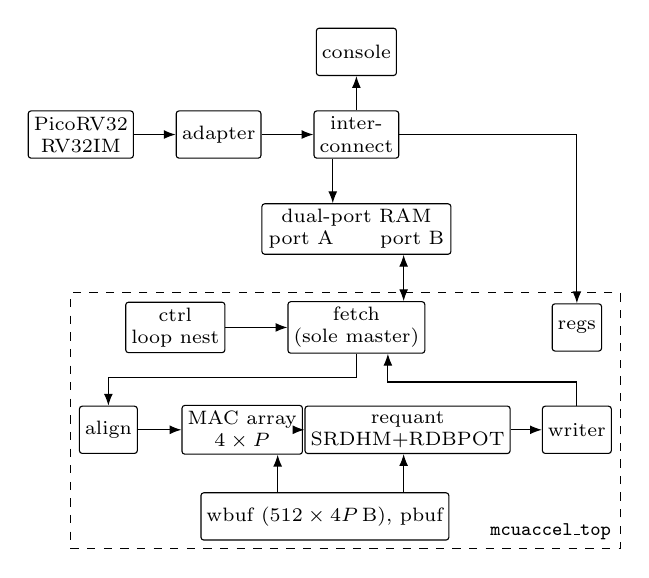
\begin{tikzpicture}[font=\scriptsize,
  b/.style={draw, rounded corners=1pt, align=center, minimum height=6mm, inner sep=2pt},
  a/.style={-{Latex[length=1.5mm]}}]
\node[b] (cpu) at (0,0) {PicoRV32\\RV32IM};
\node[b] (ad) at (1.75,0) {adapter};
\node[b] (ic) at (3.5,0) {inter-\\connect};
\node[b] (con) at (3.5,1.05) {console};
\node[b, minimum width=24mm] (ram) at (3.5,-1.2) {dual-port RAM\\port A \hspace{4mm} port B};
\node[b] (fetch) at (3.5,-2.45) {fetch\\(sole master)};
\node[b] (ctrl) at (1.2,-2.45) {ctrl\\loop nest};
\node[b] (regs) at (6.3,-2.45) {regs};
\node[b] (align) at (0.35,-3.75) {align};
\node[b] (mac) at (2.05,-3.75) {MAC array\\$\Lanes\times P$};
\node[b] (rq) at (4.15,-3.75) {requant\\SRDHM+RDBPOT};
\node[b] (wr) at (6.3,-3.75) {writer};
\node[b] (buf) at (3.1,-4.85) {wbuf ($\WbufRows\times 4P$\,B), pbuf};
\node[draw, dashed, fit=(ctrl)(fetch)(regs)(align)(wr)(buf), inner sep=3pt] (acc) {};
\node[anchor=south east, font=\scriptsize\ttfamily] at (acc.south east) {mcuaccel\_top};
\draw[a] (cpu) -- (ad); \draw[a] (ad) -- (ic); \draw[a] (ic) -- (con);
\draw[a] ([xshift=-3mm]ic.south) -- ([xshift=-3mm]ram.north);
\draw[a] (ic.east) -| (regs.north);
\draw[a, {Latex[length=1.5mm]}-{Latex[length=1.5mm]}] ([xshift=6mm]ram.south) -- ([xshift=6mm]fetch.north);
\draw[a] (ctrl) -- (fetch);
\draw[a] (fetch.south) -- ++(0,-0.3) -| (align.north);
\draw[a] (align) -- (mac); \draw[a] (mac) -- (rq); \draw[a] (rq) -- (wr);
\draw[a] (wr.north) -- ++(0,0.3) -| ([xshift=4mm]fetch.south);
\draw[a] ([xshift=-6mm]buf.north) -- ([xshift=-6mm]buf.north |- mac.south);
\draw[a] ([xshift=10mm]buf.north) -- ([xshift=10mm]buf.north |- rq.south);
\end{tikzpicture}
\caption{System and accelerator block diagram (schematic; \texttt{docs/DESIGN.md} Sec.~1). The CPU writes a descriptor address and a start bit, then polls; the accelerator reaches RAM only through its own port.}\label{fig:sys}
\end{figure}

\subsection{Bus protocol}
Every port speaks one simplified OBI-style protocol, restated from corv32's design document. A request is accepted at the end of a cycle with \code{req} and \code{gnt} both high; \code{gnt} may depend combinationally on the request. The master holds \code{req} and its payload stable until acceptance and may raise a new request only if no accepted request awaits its response or that response arrives in the same cycle, so a one-cycle-latency slave sustains one transfer per cycle with at most one outstanding request. Each accepted request receives exactly one response (\code{rvalid} for one cycle, with \code{rdata} and \code{err}) in a later cycle, in order, with no back-pressure; writes are acknowledged the same way. An error response means the access had no effect. A write is visible to any request accepted in or after the cycle of its response. All slaves in the SoC are zero-wait ($\code{gnt}=1$, response one cycle after acceptance), but every master is tested against randomly stalling slaves, and a bus checker asserts the protocol rules on every port in every test (Sec.~\ref{sec:verif}).

\subsection{Workloads}
The workloads are \texttt{mcugrad}'s two int8 per-channel models, exactly the graphs that produced the compiler's committed generated code. \texttt{mnist\_cnn} has two $3\times3$ convolutions (one and eight input channels), two max-pools, two transposes between NCHW and NHWC layouts and a fully connected layer. \texttt{cifar\_mobilenet} is a MobileNet-style network: a $3\times3$ convolution on three channels, six depthwise $3\times3$ layers alternating with six $1\times1$ convolutions, an average pool and a fully connected layer. At $P=\PDefault$ the backend maps them to \PredCommandsMnistPeight{} commands in \PredChainsMnistPeight{} chains and \PredCommandsCifarPeight{} commands in \PredChainsCifarPeight{} chains, respectively. In the software baseline's profile, the layers the accelerator can take account for \ProfileAccelShareMnist\,\% (mnist) and \ProfileAccelShareCifar\,\% (cifar) of the cycles.

\section{Accelerator Architecture}\label{sec:arch}
\subsection{Dataflow}
The datapath is output-stationary over one output pixel and a tile of $P$ output channels. For each pixel in raster order and each tile, the reduction streams activation words from RAM and weight rows from a local buffer; $P$ accumulators hold the tile's outputs, which are then requantized and written while the next tile runs.

\textbf{Row runs.} In NHWC layout, the in-bounds part of one kernel row of one output pixel, $x[i_y, i_{x0}{+}k_{x0} .. i_{x0}{+}k_{x1}{-}1, 0..C{-}1]$, is a contiguous run of bytes. The full kernel row has $\mathrm{RUN} = K_W C$ bytes, consumed as $R_Q=\lceil \mathrm{RUN}/4\rceil$ quads; run byte $b$ is the tap $(b \operatorname{div} C, b \bmod C)$. Each cycle the MAC array takes one quad of activations (\Lanes{} lanes) and one weight-buffer row of $\Lanes P$ bytes (word $p$ holding output channel $p$'s weights for the same four run bytes) and performs $\Lanes P$ multiply-accumulates. One mechanism therefore handles every channel count: a single-channel $3\times3$ layer costs one quad per kernel row rather than three taps, and three channels cost no more than four. Runs that do not start on a word boundary pass through an aligner at the cost of one priming read per kernel row. At the borders, rows outside the input are skipped, columns are clipped to the quads that contain in-bounds bytes, and lanes outside the in-bounds byte range are masked so that their $(x - z_x)$ is forced to zero, which is exactly the reference's skipped padded taps. A fully connected layer is a convolution with $H=1$, $W=N$, $K_H=K_W=1$, $C=K$ and $O=M$.

\textbf{Depthwise mode.} For a depthwise layer ($\text{groups}=C=O$, $C$ a multiple of four, aligned input), a tile is four channels; for each in-bounds tap one aligned activation word (four channels of one pixel) meets one weight word, and lane $l$ feeds only accumulator $l$, using the multipliers of output group 0. Only \Lanes{} of the $\Lanes P$ multipliers do useful work, so depthwise layers are fetch-bound by construction; reusing activations across taps would need line buffers, which we modelled but did not build (Sec.~\ref{sec:model-alt}).

\textbf{Bandwidth.} Everything goes through one \PortBits-bit port. Convolution mode reaches $\Lanes P$ multiply-accumulates per activation word, so it is port-bound when a tile's reduction is long; descriptors, weights and parameters (once per command) and output writes also consume port cycles, writes with priority over reads. The single requantizer emits one output per cycle, so a tile with fewer activation words than outputs is requantizer-bound.

\subsection{Software interface}
\textbf{Registers.} The register file is a zero-wait slave with eight word registers: an identifier, a read-only configuration word (P, lanes, buffer rows), a control register (start, clear), a status register (busy, sticky done, sticky error), the first descriptor's address, a cycle counter of the last chain, a count of completed commands and the address of a faulting access. Start sets busy at the end of the accepting cycle, so every later status read sees it until the chain ends.

\textbf{Descriptors.} A command is a \DescWords-word descriptor in RAM (Table~\ref{tab:desc}). Descriptors chain through their first word; the accelerator reads all words but the last and writes the last, the command's cycle stamp. Choosing in-memory chains over per-layer register writes (decision D8) means a chain of consecutive accelerated layers costs the CPU two stores and a poll, independent of its length; \texttt{cifar\_mobilenet}'s thirteen consecutive accelerated layers form one chain.

\begin{table}[t]\centering
\caption{Command descriptor (\DescWords{} 32-bit words; \texttt{docs/DESIGN.md} Sec.~6.2).}\label{tab:desc}
\footnotesize\setlength{\tabcolsep}{3pt}
\begin{tabular}{rlp{0.52\columnwidth}}\toprule
Word & name & content\\\midrule
0 & NEXT & next descriptor, 0 = last\\
1 & CFG & mode (conv/fc or dw), $K_H$, $K_W$, $S_H$, $S_W$, $P_H$, $P_W$\\
2--3 & IN\_HW, OUT\_HW & $H, W$; $O_H, O_W$\\
4 & CH & $C$; NCH (output channels of this command)\\
5 & RUN & RUN bytes $K_W C$; $R_Q$ (0 in dw mode)\\
6 & X\_ORIGIN & $x$ base $-P_H\,\mathrm{XROW}-P_W\,\mathrm{XPIX}$ (mod $2^{32}$)\\
7--10 & XPIX, XROW, steps & pixel, row and stride steps in bytes\\
11--12 & Y\_BASE, YPIX & first output address; output pixel step\\
13--14 & W\_BASE, WCFG & packed weights; rows to load, rows per tile\\
15 & P\_BASE & parameter records (bias, mult, shift)\\
16 & QPARAM & $z_x$, $z_y$, act\_min, act\_max (int8)\\
17 & STAMP & written by the accelerator: cycles of this command\\\bottomrule
\end{tabular}
\end{table}

\textbf{Command execution.} For each descriptor the sequencer reads the descriptor (DESC), loads the packed weight rows into the weight buffer (WLOAD) and three words per output channel into the parameter buffer (PLOAD), runs the loop nest (COMPUTE), waits until the MAC array, requantizer and writer are idle and no request is outstanding (FLUSH), writes the stamp (STAMP), and follows NEXT. The stamp counts the cycles from the first descriptor read up to the cycle before the stamp write, so per-command time is observable without a trace. On any error response the accelerator stops issuing, waits for the outstanding response, records the faulting address, resets its credits, empties the requantizer's queues, clears the writer and the MAC valids, and returns to idle with only the error bit set; a correct chain started afterwards must be bit-exact, which is tested.

\subsection{Modules}
\textbf{Fetch.} The only bus master. It arbitrates between the sequencer's read requests and the writer's (or stamp's) write requests, writes first; once a request is raised and not granted its selection is held, so the hold rule is met even if a write appears meanwhile. Every read carries a tag that returns with its response and routes it: descriptor word, weight-buffer row and word, parameter channel and field, or activation (with MAC enable, lane mask, alignment, first/last flags and weight row). Its idle output is combinational, so a wait phase ends in the cycle of the last response.

\textbf{Sequencer (ctrl).} A finite-state machine with idle, descriptor, weight-load and parameter-load phases (each with a wait state), a one-cycle pixel setup (PSETUP), a bubble-free issue state, flush, stamp and abort. Per pixel it computes the clipped kernel window and the run's first address with four 4-bit-by-32-bit shift-add products (no DSP), and in the issue state it raises a read every cycle except when the last request of a tile waits for a credit; row, tile and pixel changes cost no cycle because addresses are computed incrementally one cycle ahead. The timing in this paragraph is normative: it is the contract the RTL was built to and the model implements.

\textbf{Credits.} Two credits separate the sequencer from the requantizer, whose accumulator queue has depth two. Issuing a tile's last request takes a credit and pushes the tile's metadata (first channel, number of valid outputs $NV$, output address) to the requantizer; the requantizer returns the credit when it feeds the tile's last value into its pipeline. A post-review fix made the credit return combinational, matching the normative one-cycle loop (decision D20, Sec.~\ref{sec:method}).

\textbf{Buffers.} The weight buffer is $P$ memories of \WbufRows{} 32-bit words read in parallel (one block RAM each), written word by word during WLOAD and read with the row carried in the activation's tag, so its output is valid in the response cycle. The parameter buffer holds bias, multiplier and shift for up to \WbufRows{} channels in three memories.

\textbf{Aligner.} A register keeps the previous activation word; the quad is the current word when aligned, else the low 32 bits of the concatenation of current and previous words shifted right by eight times the alignment. A priming read only loads the register.

\textbf{MAC array.} Stage 1 forms the 9-bit signed differences $(x-z_x)$, zeroed by the lane mask, and registers the $\Lanes P$ 17-bit products; stage 2 sums each output's four products and loads or adds into its 32-bit accumulator (convolution), or adds lane $l$'s product into accumulator $l$ (depthwise); stage 3 presents the accumulators with a valid flag at a tile's last quad. Accumulators wrap modulo $2^{32}$; because the specification only uses the accumulator through $\mathrm{wrap}_{32}(\mathrm{acc} \ll \ell_s)$, a wrapping accumulator is exact for every input, and the backend additionally enforces the no-wrap bound $|b_o| + K\cdot255\cdot128 \le 2^{31}-1$.

\textbf{Requantizer.} One pipelined unit, one value per cycle, six stages (Table~\ref{tab:rq}). It implements
\begin{align}
\mathrm{SRDHM}(a,m) &= \bigl\lfloor (a m + 2^{30})/2^{31}\bigr\rfloor,\label{eq:srdhm}\\
\mathrm{RDBPOT}(x,e) &= (x \gg e) + \bigl[\rho > (\mu \gg 1) + [x<0]\bigr],\label{eq:rdbpot}\\
q &= \mathrm{RDBPOT}\bigl(\mathrm{SRDHM}(s \ll \ell_s, m),\, r_s\bigr),\nonumber\\
y &= \min\bigl(\max(q+z_y,\, a_{\min}),\, a_{\max}\bigr),\nonumber
\end{align}
where SRDHM saturates to $2^{31}-1$ in the single case $a=m=-2^{31}$, $\mu = 2^e-1$, $\rho = x \mathbin{\&} \mu$, $s = \mathrm{wrap}_{32}(\mathrm{acc}+b)$, $\ell_s=\max(\mathrm{shift},0)$, $r_s=\max(-\mathrm{shift},0)$, $\gg$ arithmetic. The closed form of (\ref{eq:srdhm}) equals gemmlowp's truncating-nudge form; the sum with $z_y$ is formed in 33 bits and compared signed before the clamp, because a 32-bit sum could wrap where the specification clamps. The 32$\times$32 multiply maps to four \texttt{MULT18X18D}.

\begin{table}[t]\centering
\caption{Requantizer pipeline (one value per cycle).}\label{tab:rq}
\footnotesize\setlength{\tabcolsep}{3pt}
\begin{tabular}{ll}\toprule
Stage & operation\\\midrule
S0 & read parameters of channel $ch_0+i$; select accumulator $i$\\
S1 & $s=\mathrm{wrap}_{32}(\mathrm{acc}+b)$; $a=\mathrm{wrap}_{32}(s\ll\ell_s)$\\
S2 & 64-bit product $a\cdot m$\\
S3 & SRDHM, with the $-2^{31}\cdot-2^{31}$ special case\\
S4 & RDBPOT by $r_s$ (round half away from zero)\\
S5 & 33-bit $+z_y$, signed clamp, output byte\\\bottomrule
\end{tabular}
\end{table}

\textbf{Writer.} It assembles consecutive output bytes of a tile into a word with byte enables and hands the word to a one-entry pending write when the word is full or the tile ends; it back-pressures the requantizer, which then freezes all its stages.

\textbf{Pipeline timing.} Relative to the response cycle $r$ of an activation read, the products are registered at the end of $r$, the accumulation at the end of $r+1$, and at a tile's last quad the accumulators enter the requantizer's queue at the end of $r+2$; with a response latency $\lambda$, issue to accumulator availability takes $\lambda+3$ cycles. This latency, the two credits and the requantizer's rate are the three quantities the cost model needs besides the port.

\section{Backend and Driver}\label{sec:backend}
\subsection{From compiler graph to commands}
The backend (\texttt{backend/mcuaccel\_backend}) consumes the int8 graph built by \texttt{mcugrad}'s own pipeline (trained weights, tracing, optimisation, calibration, per-channel quantisation) and checks that emitting it with \texttt{mcugrad}'s code generator reproduces the committed \texttt{model.c} byte for byte, so the accelerated and baseline builds start from the same model. A support check accepts convolutions with one group and kernel, stride and padding within the descriptor's fields (padding smaller than the kernel), depthwise convolutions with a channel count divisible by four, and matrix multiplications as $1\times1$ convolutions; everything else (pooling, transposes, padding, additions, softmax, and any convolution outside the envelope) falls back to the compiler's kernel, pasted byte for byte as the compiler emits it. Two optional passes (dropping an identity transpose, folding a transpose into fully connected weights) exist but are pre-registered as off in every scored build.

\textbf{Packing.} In convolution mode, for a command covering output channels $o_s..o_s{+}\mathrm{NCH}{-}1$ with $N_T=\lceil \mathrm{NCH}/P\rceil$ tiles, weight row $r = (tK_H + k_y)R_Q + j$ holds, in word $p$ and byte $l$, the weight $w[o_s{+}tP{+}p][k_y][b \operatorname{div} C][b \bmod C]$ with $b=4j+l$, or zero past the run or past NCH. A command loads $N_T K_H R_Q$ rows of $P$ words. In depthwise mode, row $r = gK_HK_W + k_yK_W + k_x$ is one word holding the tap weights of channels $c_0{+}4g..c_0{+}4g{+}3$. Each output channel has a three-word parameter record: the graph's unfolded int32 bias, the multiplier and the shift, of which the hardware keeps the low six bits sign-extended. The accelerator computes the unfolded form, with the bias added in the requantizer; \texttt{mcugrad}'s folded bias would need per-pixel padded-tap corrections in hardware (decision D10).

\textbf{Splitting.} A command's weights must fit \WbufRows{} buffer rows and its channels the parameter buffer. Convolutions are split over output channels into commands of $P\lfloor \WbufRows/(K_H R_Q)\rfloor$ channels that share the input and offset the output, weight and parameter bases; depthwise layers are split over channels into commands of $4\lfloor \WbufRows/(K_HK_W)\rfloor$; a layer whose single tile needs more rows than the buffer falls back to software. Because a command holds $P\lfloor \WbufRows/(K_HR_Q)\rfloor$ channels, splits occur in the two workloads only at small $P$: \MOneRowsPone{}, \MOneRowsPtwo{} and \MOneRowsPfour{} scored commands at $P=1,2,4$ against \MOneRowsPeight{} unsplit commands at $P=8$ and $16$.

\textbf{Guards.} The aligner and border clipping may read a few bytes outside a tensor; they are masked and never written. The backend cannot see where the network input will live, so this is enforced as a link-time property: the linker script pads both RAM edges and asserts that no section lies near them. The backend also forbids overlap of a command's input and output ranges.

\subsection{Executor}
A pure-Python executor of the descriptor semantics (\texttt{exec.py}) is the reference for the RTL's functional behaviour. Where the design text left room for interpretation, the executor fixes it (for example, the accumulator wraps per tile, the priming read happens only when misaligned, split descriptors are contiguous), and its docstring lists every such resolution; the RTL is required to match the executor, and the executor is tested equal to \texttt{mcugrad}'s integer operators on seeded random layers and forced splits. Its optional trace (every activation read with address, mask, alignment and flags, and every tile's metadata) is the golden request stream for the sequencer's unit test, which checks addresses, tags and order but never cycle counts, so the RTL's timing is not tuned to the model through the tests.

\subsection{Generated code and driver}
The emitter writes a \texttt{model.c} with the same \texttt{model\_run} interface as the compiler's: packed weights and parameters as constant arrays, one descriptor array per chain, and per-chain functions. All address fields are emitted as offsets; a bind step on the first call adds the real bases (next pointers, input, output, weight and parameter addresses), and each later call re-patches only the fields that depend on the network's input and output (the first layer's input origin and the last layer's output base). The emitted file records its $P$, and bind compares it with the accelerator's configuration register, so firmware built for one width never silently runs on another.

The driver (\texttt{sw/driver}) writes the descriptor address, writes start, polls the busy bit, and on error writes a failure code to the console and stops. Compiler barriers before the register writes and after the poll loop prevent cached arena values from being reused across a chain, and addresses are computed in \code{uintptr\_t} rather than through out-of-object pointer arithmetic. The driver was written and measured on a stub accelerator before the model was frozen, so the model's driver constants are measurements: \DrvChain{} cycles per chain call and \DrvPatch{} per patched field.

\section{Cost Model}\label{sec:model}
The model (\texttt{model/m1.py}; normative text in \texttt{docs/DESIGN.md} Sec.~7) is a loop nest over the output pixels and channel tiles of a command with one closed form per tile. It was implemented from the design text, and a reviewer recomputed three layers by hand before it was frozen.

\subsection{Per-pixel geometry}
For output pixel $(o_y,o_x)$ the sequencer computes, in its setup cycle,
\begin{align}
i_{y0} &= o_y S_H - P_H,\qquad i_{x0} = o_x S_W - P_W,\nonumber\\
k_{y0} &= \max(0,-i_{y0}),\qquad k_{y1}=\min(K_H,\, H-i_{y0}),\nonumber\\
k_{x0} &= \max(0,-i_{x0}),\qquad k_{x1}=\min(K_W,\, W-i_{x0}),\nonumber\\
b_0 &= k_{x0}C,\quad b_1 = k_{x1}C,\quad j_0 = \lfloor b_0/4\rfloor,\quad j_1=\lceil b_1/4\rceil.\label{eq:geom}
\end{align}
In convolution mode a kernel row $k_y$ whose run starts at address $A_{k_y}+4j_0$ costs
\begin{equation}
R_{\mathrm{row}}(k_y) = (j_1 - j_0) + \bigl[(A_{k_y}+4j_0) \bmod 4 \ne 0\bigr]\label{eq:rrow}
\end{equation}
activation words (the bracket is the priming read), and the pixel needs $R = \sum_{k_y=k_{y0}}^{k_{y1}-1} R_{\mathrm{row}}(k_y)$ words per tile. In depthwise mode $R = (k_{y1}-k_{y0})(k_{x1}-k_{x0})$. Activations are re-read for every tile.

Tile $t$ has $NV_t = \min(P, \mathrm{NCH}-tP)$ valid outputs in convolution mode and $NV_t=4$ in depthwise mode, and its outputs need
\begin{equation}
W_t = \bigl\lceil \bigl((y_t \bmod 4) + NV_t\bigr)/4\bigr\rceil\label{eq:wt}
\end{equation}
word writes at output address $y_t$. These writes are issued while later tiles are fetched; each steals one port slot from them.

\subsection{Tile, pixel, command and chain}
Let $\lambda$ be the cycles per bus transaction ($\lambda=1$ on the zero-wait RAM), $D=\DescWords$ the descriptor length, $W_{\mathrm{w}}$ the weight words loaded ($N_T K_H R_Q P$ in convolution mode, $(\mathrm{NCH}/4)K_HK_W$ in depthwise mode) and NCH the command's output channels. Then
\begin{align}
T_{\mathrm{tile}}(t) &= \max\Bigl(\lambda(R{+}W_t),\; NV_t,\; \Bigl\lceil\tfrac{NV_t+\lambda+3}{2}\Bigr\rceil\Bigr),\label{eq:tile}\\
T_{\mathrm{pix}} &= 1+\textstyle\sum_t T_{\mathrm{tile}}(t),\label{eq:pix}\\
T_{\mathrm{cmd}} &= \bigl[(D{-}1)\lambda+1\bigr] + \bigl[\lambda W_{\mathrm{w}}+1\bigr] + \bigl[3\lambda\,\mathrm{NCH}+1\bigr]\nonumber\\
&\quad + \textstyle\sum_{\mathrm{pix}} T_{\mathrm{pix}} + \bigl[2\lambda+10+NV_{\mathrm{last}}\bigr],\label{eq:cmd}\\
T_{\mathrm{chain}} &= \textstyle\sum_{\mathrm{cmd}} (T_{\mathrm{cmd}}+\lambda+1) + 2.\label{eq:chain}
\end{align}
The three terms of (\ref{eq:tile}) are the port bound (the tile's reads plus the previous tile's writes), the requantizer bound (one output per cycle), and the two-credit latency bound for tiles with few outputs: with two result slots and an issue-to-accumulator latency of $\lambda+3$, two tiles must cover the latency plus the requantizer's drain. The $1$ in (\ref{eq:pix}) is the setup cycle. The brackets of (\ref{eq:cmd}) are the descriptor, weight and parameter loads (each with its one-cycle wait), the compute phase and the final drain (the constant is the requantizer's six-stage latency plus four cycles of hand-off); $T_{\mathrm{cmd}}$ is exactly what the accelerator writes as the stamp. Equation (\ref{eq:chain}) adds the stamp write per command and the start and done cycles visible to the CPU.

\subsection{Closed forms for the workloads}
With aligned tensors, $\lambda=1$ and $NV=P$ when $\mathrm{NCH}\ge P$:
\begin{itemize}\setlength{\itemsep}{1pt}
\item $1\times1$ convolution with $C$ and $O$ multiples of four and of $P$ (\texttt{cifar} ops 2, 4, \dots, 12): no borders, $R=C/4$, $W=\lceil P/4\rceil$, and
$T_{\mathrm{compute}} = O_HO_W\bigl(1 + \tfrac{O}{P}\max(\tfrac{C}{4}+\lceil\tfrac{P}{4}\rceil,\,P,\,\lceil\tfrac{P+4}{2}\rceil)\bigr)$. The layer is port-bound when $C$ exceeds about $3P$ and requantizer-bound below.
\item $3\times3$ depthwise with padding one (\texttt{cifar} ops 1, 3, \dots, 11): $W=1$, $NV=4$, and $T_{\mathrm{compute}} = O_HO_W + \tfrac{C}{4}\sum_{\mathrm{pix}}\max(R+1,4)$, independent of $P$.
\item $3\times3$ convolution with $C\in\{1,3,8\}$ (\texttt{mnist} ops 1, 3; \texttt{cifar} op 0): $R$ from (\ref{eq:rrow}); eight channels are always aligned, one and three channels pay the priming word on three of four alignments.
\item Fully connected with $K$ inputs and $\lceil 10/P\rceil$ tiles: $T_{\mathrm{compute}} = 1 + \sum_t \max(K/4 + W_t, NV_t, \lceil (NV_t+4)/2\rceil)$, and WLOAD dominates.
\end{itemize}
These forms already state the mechanism of C5: in convolution mode the port term still falls as $1/P$ because activations are re-fetched per tile, so the sweep should flatten because of the depthwise layers (fixed four multiply-accumulates per cycle), the single requantizer and the weight load (roughly constant in $P$), not because the \PortBits-bit port saturates.

\subsection{Whole network}
The predicted accelerated \texttt{model\_run} is the sum over chains of $T_{\mathrm{chain}} + t_{\mathrm{drv}} + n_{\mathrm{patch}}\,t_{\mathrm{patch}}$, with the measured $t_{\mathrm{drv}}=\DrvChain$ and $t_{\mathrm{patch}}=\DrvPatch$, plus the measured baseline cycles of every operator that stays in software, plus the \BenchWindow-cycle bench window present in both builds. The software term is a measurement carried through to obtain a predicted speedup; claim C4b scores only the accelerator-plus-driver part, so the prediction cannot be right merely because its largest term was measured. At $P=\PDefault$ the frozen prediction is \PredCfourBMnistPeight{} accelerator-plus-driver cycles for mnist and \PredCfourBCifarPeight{} for cifar, with \PredSwCyclesMnistPeight{} and \PredSwCyclesCifarPeight{} software cycles, i.e.\ software at \PredSwShareMnistPeight\,\% and \PredSwShareCifarPeight\,\% of the predicted run.

\subsection{Alternative architectures (modelled, not built)}\label{sec:model-alt}
Before choosing the design, the model was evaluated for two alternatives with the same multipliers and port. \emph{Line buffer} (``lb''): each in-bounds input row is streamed once per output row and tile into a $K_H$-row buffer; in depthwise mode the multipliers become four channels times up to $P$ adjacent output pixels. \emph{Accumulator memory} (``acc''): activations are fetched once per pixel and all tiles accumulate in a memory, $T_{\mathrm{pix}} = 1 + \max(\lambda(R + \sum_t W_t),\, \sum_t\sum_{k_y}(j_1-j_0),\, \sum_t NV_t)$. At $P=\PDefault$ the frozen predictions of summed stamps per inference are \PredStampCifarPeight{} (built), \PredStampLbCifarPeight{} (lb) and \PredStampAccCifarPeight{} (acc) for cifar, and \PredStampMnistPeight, \PredStampLbMnistPeight{} and \PredStampAccMnistPeight{} for mnist (Fig.~\ref{fig:m1}). The output-stationary design was built because it needs no line buffers and handles every channel count with one mechanism (decision D9); the predicted gain of the line buffer comes almost entirely from the depthwise layers.

\begin{figure*}[t]\centering
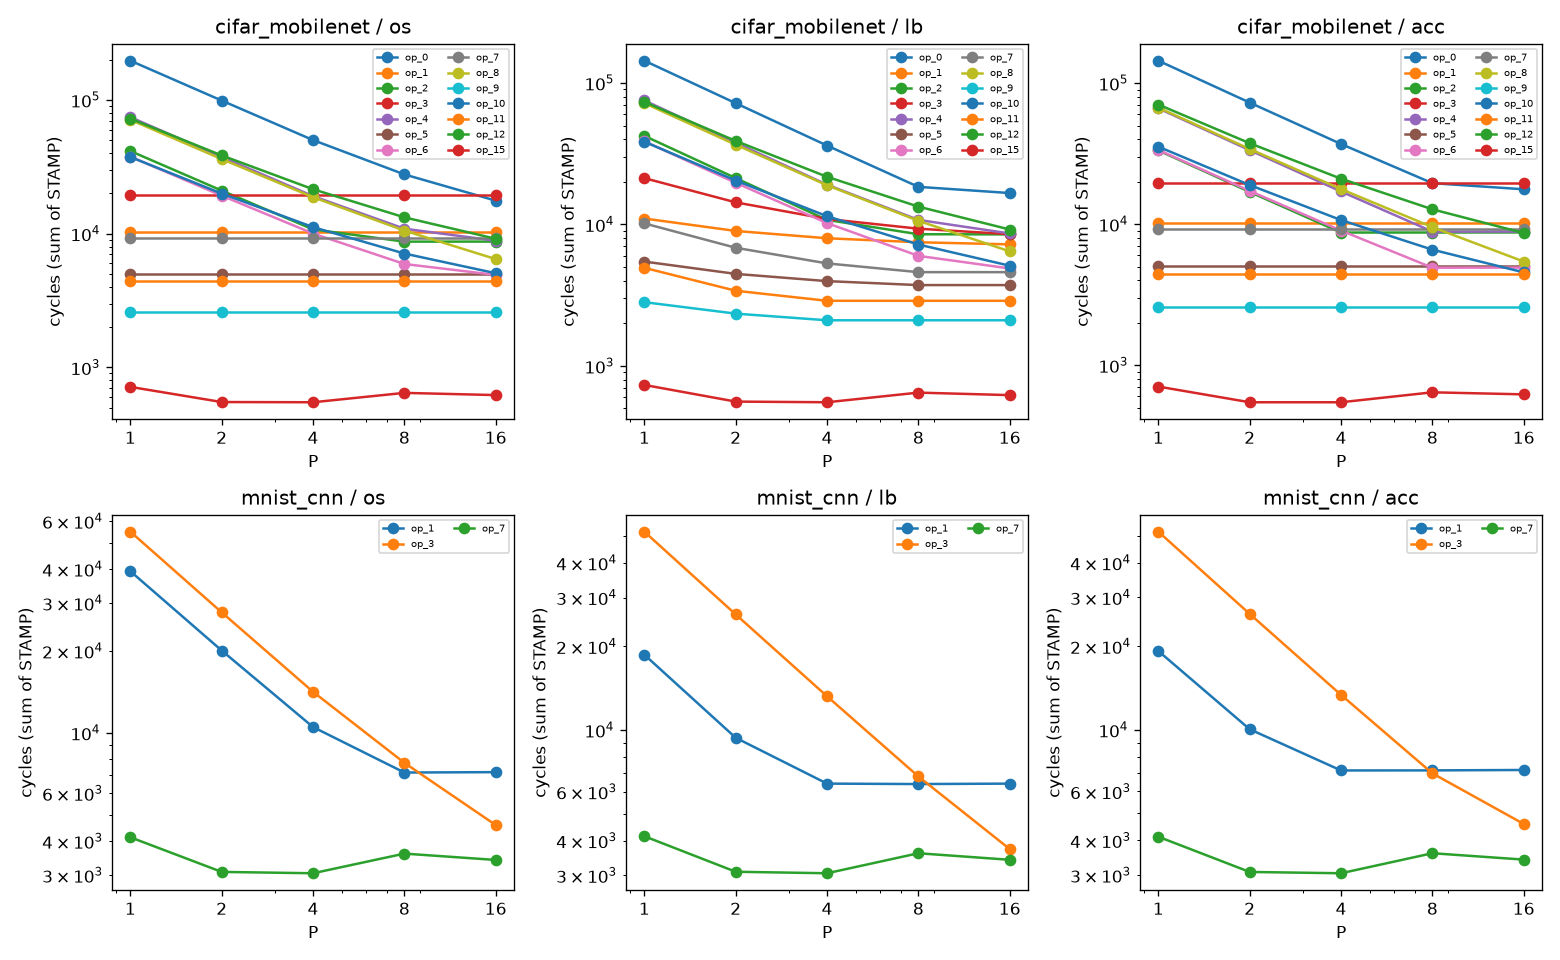
\includegraphics[width=0.92\textwidth]{m1_cycles_vs_P.png}
\caption{Frozen per-command predictions (tag \texttt{m1}, unchanged since): predicted stamp cycles per command versus $P$ for the built output-stationary design (os) and the two modelled alternatives (lb, acc). Flat lines are depthwise commands; the cifar fully connected command rises slightly at $P=8$ because its weight load grows with the tile.}\label{fig:m1}
\end{figure*}

\subsection{Registered biases}\label{sec:biases}
Before freezing, the design document listed where the model is known to be wrong and by how much (the same list is inside the frozen summary file):
\begin{itemize}\setlength{\itemsep}{1pt}
\item The setup cycle is hidden behind the requantizer where a layer is requantizer- or credit-bound; the model keeps it. Named commands were given a registered over-prediction of a few percent, all others less than \BiasDefault\,\% (Table~\ref{tab:exceed}, last column).
\item The drain term counts the last tile's writes and outputs in both the tile and the drain, over-predicting by $2+W_{\mathrm{last}}$ cycles per command.
\item The wait phases are exact only if the fetch unit's idle signal is combinational, as specified.
\item The driver constants omit the per-call bind check and the poll loop's phase wait, a few tens of cycles per network.
\item The C4b measurement interval contains profiling instrumentation and call overhead that the prediction does not.
\item The output alignment of the final layer is assumed zero.
\end{itemize}
Each item states a direction and a magnitude, so a measured error can be checked against it (Sec.~\ref{sec:results-c4}).

\section{Methodology}\label{sec:method}
\subsection{Pre-registration protocol}
Tag \texttt{m1} precedes in git history every commit that adds a datapath or sequencer to the accelerator RTL; only a register-file stub that sets done without computing existed before it. The model is not changed to match the RTL; post-hoc model fixes would be reported beside the frozen predictions, which remain the scored ones (none was made). The RTL is not tuned to the model either: it is scored as it stood at its first full stamp measurement, and every later change that alters a stamp is logged with before and after values. Scored predictions are the rows of \texttt{m1\_predictions.csv} for the built architecture, \MOneRowsPeight{} commands at $P=\PDefault$ and \MOneRows{} over the sweep, joined on network, operator, $P$ and split index; a measured command without a predicted row, or vice versa, counts as a violation. The tag's commit and the file hash were made public at \PreregUrl{} on \PreregDate{}. That server timestamp shows the predictions existed by that date; the full history was published in one push, so their order before the datapath commits rests on the git history.

\subsection{Timing protocol}
Inference time is the \code{rdcycle} interval around \texttt{model\_run} on the SoC CPU, including software layers, descriptor patching, polling and driver cost, over \BaselineImagesMnist{} fixed test images and \BaselineRunsMnist{} timed runs after one warm-up (decision D17: the simulator is deterministic, so more runs add only wall time). We report the median over runs of the per-run median over images, with the minimum and maximum over images. The bench window inside the interval costs \BenchWindow{} cycles in both builds. Simulation runs at a nominal \ClockMHzMnist{}\,MHz, which only converts cycles to time; cycles are the claimed unit.

Per-command time is the stamp. Per-network accelerator-plus-driver time for C4b is measured in one instrumented profile build per network as the \texttt{model\_run} interval minus the bench window minus the sum of the fallback operators' \code{rdcycle} intervals, per image, median over the timed images. Stamps per command are collected in a separate build that prints them; the stamp is a hardware value, so it does not depend on the instrumentation.

\subsection{Baseline and fairness}
The baseline is \texttt{mcugrad}'s generated \texttt{model.c} with its own kernels, compiled with the same GCC flags (\code{-O2 -march=rv32im\_zicsr}) and run on the same SoC with the accelerator present and idle, with the same images and the same bench harness. The accelerated build differs only in the operators the accelerator takes. Fairness requires the fallback operators to be identical machine code in both builds. Text identity was not enough: GCC inlined and register-allocated the kernels differently depending on which other operators a file contained, so the same operator cost a few cycles more or less in the two builds. Both builds therefore pin inlining at build time (decision D19): every kernel is \code{always\_inline} into its one operator function and every operator function is \code{noinline}, so each fallback operator is compiled from its own text alone; the source text is unchanged and the attributes are added by a build script. A second difference, a register move landing inside the first profiled operator because a bind call clobbered the argument register, was removed in the emitter. Identity is checked by measurement, not by object-code hash: on the same inferences, every fallback operator reports identical per-inference cycles in the two profile builds. A shared non-inlined kernel file was also tried and rejected because it slowed both builds by removing constant propagation.

\subsection{Deviations after the freeze}
Two logged changes altered measured cycles; neither changed a frozen prediction or a threshold (values in \texttt{results/deviations.json}, written by a script that checks them against the decision log).

\emph{D19, the fairness fix.} Pinning inlining moved the baseline from \DevBaseBeforeMnist{} to \BaselineCyclesMnist{} cycles (mnist) and from \DevBaseBeforeCifar{} to \BaselineCyclesCifar{} (cifar), and the accelerated $P=\PDefault$ build from \DevAccelBeforeMnist{} to \MeasCyclesMnistPeight{} and from \DevAccelBeforeCifar{} to \MeasCyclesCifarPeight{}; the measured speedup moved from \DevSpeedupBeforeMnist$\times$ to \DevSpeedupAfterMnist$\times$ (mnist) and from \DevSpeedupBeforeCifar$\times$ to \DevSpeedupAfterCifar$\times$ (cifar). No accelerator cycle changed. The mnist change is large because its accelerated runtime is dominated by pooling and transposes, which the earlier inlining compiled badly. Because the frozen speedup predictions used the pre-fix baselines and pre-fix fallback cycles, we add a post-hoc rescoring (Sec.~\ref{sec:results-c1}).

\emph{D20, the credit loop.} A red-team review of the RTL found a blocker (a credit returned during abort left the sequencer with three credits) and a credit return with one register stage more than the normative timing. The return was made combinational to match the design text written before the freeze; the model was not consulted. No full stamp measurement existed before the change, so the scored RTL is the fixed one. Smoke runs on the earlier RTL gave a C4b error of \DevCfourBErrBeforeMnist\,\% (mnist) and \DevCfourBErrBeforeCifar\,\% (cifar), against \DevCfourBErrAfterMnist\,\% and \DevCfourBErrAfterCifar\,\% on the scored RTL.

\section{Verification}\label{sec:verif}
\subsection{Unit level}
Every accelerator and SoC module has cocotb tests on Verilator. A bus checker attached to every master and slave port in every test asserts the protocol rules each cycle (hold, one outstanding, response count and order, no response without request); the slave model is zero-wait or randomly stalling (random grant and response latency, seeded). The requantizer is tested against the specification's \code{requant} and clamp on directed edge cases (extreme accumulators, multipliers and shifts, the $-2^{31}\cdot-2^{31}$ case, equal clamp bounds, zero points that push the sum past 32 bits) and on random vectors, with back-pressure. The MAC array is tested in both modes for several $P$, the aligner on all alignments, the writer on random start alignments, tile sizes and acceptance delays, the fetch unit on random read/write mixes against stalling slaves, and the sequencer's request stream against the executor's trace.

\subsection{Accelerator level (C2a)}
A seeded random layer generator draws convolution, depthwise and fully connected layers with kernels, strides, padding, spatial sizes and channel counts over the descriptor's envelope (including some layers with more than \WbufRows{} output channels to force splits), full-range int8 activations and weights, random zero points, biases up to the no-wrap bound, multipliers in the normal and the full int32 range, shifts over the whole legal range, random clamps, input and output base alignments from zero to three bytes, and randomly stalling slaves. The backend packs each layer and builds its descriptors, the RTL runs them from a RAM model, and the output bytes are compared with the specification's layer functions. The campaign ran \MThreePerP{} layers at each width $P\in\{\MeasCtwoAPs\}$, \MeasCtwoALayers{} in total, with \MeasCtwoAMismatch{} mismatching bytes (C2a asks for \RandomLayers{} layers; the campaign ran that set at every width). It also ran \MThreeChainsTotal{} random descriptor chains, \MThreeErrorsTotal{} runs with an error response injected mid-command (checking the error bit, the faulting address, the absence of further bus accesses, and bit-exactness of a following correct chain) and \MThreeBusyTotal{} start-while-busy checks, with \MThreeProblemsTotal{} problems in total (RTL at commit \texttt{\MThreeCommit}).

\subsection{Network level (C2b, C2c)}
For C2b the int8 graph is run node by node for \MeasCtwoBImages{} images per network, accelerated nodes on the RTL through the backend's descriptors (\MThreeNodesMnist{} and \MThreeNodesCifar{} accelerated node executions) and other nodes through the specification's operators, and every intermediate tensor is compared with the simulator: \MeasCtwoBMismatch{} mismatches. For C2c both firmware builds run on the full SoC for \MeasCtwoCImages{} test images per network and print their output bytes, which are compared with the integer simulator (\MeasCtwoCMismatch{} mismatching bytes) and with the baseline firmware's outputs: \MeasCtwoCBaseMnist{} for mnist and \MeasCtwoCBaseCifar{} for cifar. The test sets are regenerated from the compiler's quantized images with 4-byte-aligned arrays, because the full test sets do not fit the simulated RAM.

\subsection{Backend}
The executor is tested equal to the specification on seeded random layers (\texttt{MCUACCEL\_SEEDS} sets the count) and on forced splits; packing, descriptor fields and the worked example of the design document are tested directly. The emitted C is built with warnings as errors for the host and run against a host model of the accelerator, giving a host-side bit-exactness check of the generated code before any RTL is involved, and a textual test checks that every fallback kernel in the accelerated build is the baseline's text.

\section{Results}\label{sec:results}
\subsection{Baseline and Amdahl decomposition}
Table~\ref{tab:base} gives the software baseline. The runs are deterministic: the \BaselineRunsMnist{} run medians are identical in every build, and the spread is across images only.

\begin{table}[t]\centering\caption{Software baseline on the SoC (cycles per inference over \BaselineImagesMnist{} images).}\label{tab:base}
\tabtodo\begin{tabular}{lrrr}\toprule
Network & median & min & max\\\midrule
\texttt{mnist\_cnn} & \BaselineCyclesMnist & \BaselineMinMnist & \BaselineMaxMnist\\
\texttt{cifar\_mobilenet} & \BaselineCyclesCifar & \BaselineMinCifar & \BaselineMaxCifar\\\bottomrule
\end{tabular}\end{table}

Table~\ref{tab:ops} decomposes both builds per operator at $P=\PDefault$ from the profile builds. In the accelerated mnist run the chains account for \AmdahlChainShareMnist\,\% of the cycles and the fallback operators (two max-pools and two transposes) for \AmdahlFallbackShareMnist\,\%; in cifar the chains account for \AmdahlChainShareCifar\,\% and the single average pool for \AmdahlFallbackShareCifar\,\%. The fallback operators bound the speedup even for an accelerator that takes zero cycles: \AmdahlCeilingMnist$\times$ for mnist and \AmdahlCeilingCifar$\times$ for cifar. Measured mnist is already close to its ceiling, so no accelerator change can move it much; the remaining work is in software.

\begin{table}[t]\centering
\caption{Per-operator cycles per inference, baseline versus accelerated at $P=\PDefault$ (profile builds, instrumentation included; cifar's chain includes the depthwise layers). Each column is a mean over its own build's profiled images, and the two image sets differ, so the data-dependent pooling operators differ by a few cycles here although they are cycle-identical on the same inferences (Sec.~\ref{sec:method}).}\label{tab:ops}
\footnotesize% generated by experiments/make_macros.py from results/baseline_profile_*.json and m5_profile_*_P8.json; do not edit
\begin{tabular}{llrr}\toprule
net & op (kind) & baseline & accel.\ $P{=}8$\\\midrule
mnist & 0 (transpose) & 23,344 & 23,344 \\
mnist & 1 (conv, chain) & 3,352,201 & 6,437 \\
mnist & 2 (maxpool) & 116,915 & 116,904 \\
mnist & 3 (conv, chain) & 7,584,637 & 7,797 \\
mnist & 4 (maxpool) & 60,748 & 60,753 \\
mnist & 5 (transpose) & 23,952 & 23,952 \\
mnist & 7 (matmul, chain) & 221,704 & 3,682 \\
\midrule
cifar & 0--12 (conv, chain) & 69,069,151 & 133,942 \\
cifar & 13 (avgpool) & 62,764 & 62,764 \\
cifar & 15 (matmul, chain) & 38,020 & 730 \\
\bottomrule
\end{tabular}

\end{table}

\subsection{Speedup (C1, C1b)}\label{sec:results-c1}
Table~\ref{tab:speed} compares the frozen prediction with measurement over the sweep. At $P=\PDefault$ the measured speedups are \MeasSpeedupMnistPeight$\times$ and \MeasSpeedupCifarPeight$\times$: C1 is \VerdictCone{} and C1b is \VerdictConeB. The frozen predicted speedups (\PredSpeedupMnistPeight$\times$ and \PredSpeedupCifarPeight$\times$) were computed against the pre-D19 baselines and fallback cycles (Sec.~\ref{sec:method}), so they are not comparable one to one with the measured columns. The post-hoc row replaces only the software term: the frozen accelerator-plus-driver prediction, plus the measured fallback-operator cycles of the accelerated profile build (\PostHocFallbackMnist{} and \PostHocFallbackCifar{}), plus the bench window. It gives \PostHocCyclesMnist{} and \PostHocCyclesCifar{} cycles against measured \MeasCyclesMnistPeight{} and \MeasCyclesCifarPeight{}, i.e.\ \PostHocSpeedupMnist$\times$ and \PostHocSpeedupCifar$\times$. This row is post hoc by construction and is not scored.

\begin{table}[t]\centering\caption{End-to-end speedup versus $P$: frozen prediction (against pre-D19 baselines) and measurement; last row: post-hoc rescoring at $P=\PDefault$ in the prediction columns.}\label{tab:speed}
\small\tabtodo\begin{tabular}{rrrrr}\toprule
& \multicolumn{2}{c}{mnist} & \multicolumn{2}{c}{cifar}\\
$P$ & pred. & meas. & pred. & meas.\\\midrule
\row{one}\row{two}\row{four}\row{eight}\row{sixteen}\midrule
\PDefault{} post-hoc & \PostHocSpeedupMnist & \MeasSpeedupMnistPeight & \PostHocSpeedupCifar & \MeasSpeedupCifarPeight\\\bottomrule
\end{tabular}\end{table}

\subsection{Bit-exactness (C2)}
Random layers: \MeasCtwoALayers{} over the widths $P\in\{\MeasCtwoAPs\}$, \MeasCtwoAMismatch{} mismatching bytes (C2a \VerdictCtwoA). Intermediate tensors: \MeasCtwoBImages{} images per network, \MeasCtwoBMismatch{} mismatches. Full SoC: \MeasCtwoCImages{} images per network, \MeasCtwoCMismatch{} mismatching bytes against the integer simulator, and \MeasCtwoCBaseMnist{} (mnist) and \MeasCtwoCBaseCifar{} (cifar) against the baseline firmware's outputs (C2c \VerdictCtwoC).

\subsection{Prediction accuracy (C4)}\label{sec:results-c4}
Table~\ref{tab:cmdP} summarises C4a per width and Table~\ref{tab:cmd} lists every command at $P=\PDefault$. Over all \MeasCfourRows{} scored rows the maximum absolute error is \MeasCfourMaxErr\,\%, the median signed error \MeasCfourMedianErr\,\%, and \MeasCfourViolations{} rows exceed the \ThreshFourA\,\% tolerance: C4a is \VerdictCfourA. Per network at $P=\PDefault$, the measured accelerator-plus-driver time is \MeasCfourBMnist{} cycles (mnist) and \MeasCfourBCifar{} (cifar) against predicted \PredCfourBMnistPeight{} and \PredCfourBCifarPeight{}, signed errors \MeasCfourBErrMnist\,\% and \MeasCfourBErrCifar\,\%, within the \ThreshFourB\,\% tolerance. Fig.~\ref{fig:p} overlays the measurement on the frozen prediction.

The error is small and almost symmetric at $P\le4$ and grows at $P=8$ and $16$, where the requantizer term of (\ref{eq:tile}) becomes comparable to the port term on narrow layers. The median signed error is positive at every width: the model over-predicts slightly, as the registered biases said it would.

\begin{table}[t]\centering
\caption{C4a per width: scored commands, maximum absolute and median signed error (\%).}\label{tab:cmdP}
\begin{tabular}{rrrr}\toprule
$P$ & rows & max $|$err$|$ & median err\\\midrule
\crow{one}\crow{two}\crow{four}\crow{eight}\crow{sixteen}\bottomrule
\end{tabular}
\end{table}

\begin{table}[t]\centering\caption{Per-command cycles at $P=\PDefault$ (pred.\ from tag \texttt{m1}; meas.\ = median stamp over the timed images).}\label{tab:cmd}
\footnotesize
% generated by experiments/make_macros.py from results/m1_predictions.csv (tag m1); do not edit
\tabtodo\begin{tabular}{llllrr}\toprule
net & op & kind & K & pred. & meas.\\\midrule
mnist & 1 & conv & 3x3 & 7,144 & 6,356 \\
mnist & 3 & conv & 3x3 & 7,756 & 7,715 \\
mnist & 7 & fc & 1x1 & 3,596 & 3,594 \\
cifar & 0 & conv & 3x3 & 27,724 & 27,029 \\
cifar & 1 & dw & 3x3 & 10,236 & 10,203 \\
cifar & 2 & conv & 1x1 & 8,712 & 8,452 \\
cifar & 3 & dw & 3x3 & 19,436 & 19,376 \\
cifar & 4 & conv & 1x1 & 10,888 & 10,883 \\
cifar & 5 & dw & 3x3 & 5,012 & 4,995 \\
cifar & 6 & conv & 1x1 & 5,928 & 5,923 \\
cifar & 7 & dw & 3x3 & 9,204 & 9,176 \\
cifar & 8 & conv & 1x1 & 10,536 & 10,469 \\
cifar & 9 & dw & 3x3 & 2,580 & 2,571 \\
cifar & 10 & conv & 1x1 & 7,096 & 7,077 \\
cifar & 11 & dw & 3x3 & 4,436 & 4,424 \\
cifar & 12 & conv & 1x1 & 13,240 & 13,237 \\
cifar & 15 & fc & 1x1 & 644 & 642 \\
\bottomrule
\end{tabular}

\end{table}

\begin{figure*}[t]\centering
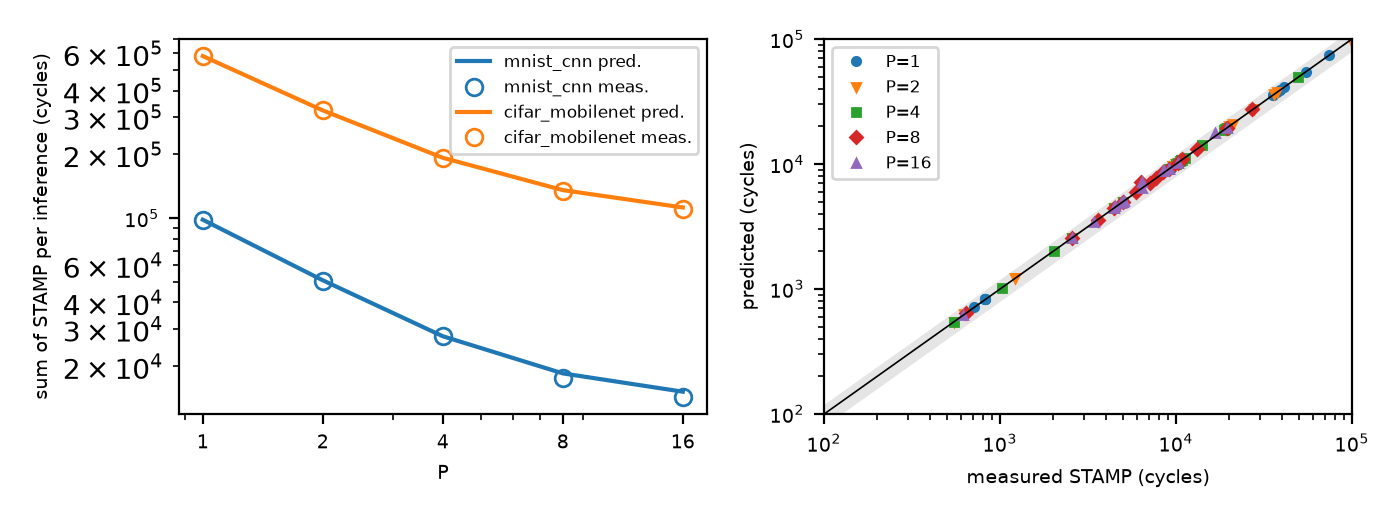
\includegraphics[width=0.8\textwidth]{m6_pred_vs_meas.png}
\caption{Frozen prediction (tag \texttt{m1}, output-stationary architecture) against measurement. Left: summed stamps per inference versus $P$ (line: prediction, circles: measurement). Right: every scored command, predicted versus measured cycles; the band is $\pm\ThreshFourA\,\%$.}\label{fig:p}
\end{figure*}

\textbf{Rows over the registered bias.} \NExceed{} scored rows exceed their registered bias by more than \ExceedMargin{} percentage points (Table~\ref{tab:exceed}); all are inside the tolerance, so C4a is unchanged, but the registered bias list was wrong for them. The root cause was found after measurement by probing the RTL (post hoc; \texttt{experiments/probe\_tie.py}, \texttt{results/m6\_tie\_probe.json}), and all \TieNProbed{} rows were probed. Equation (\ref{eq:pix}) adds the setup cycle to the tile terms, but the RTL grants the writer's pending write of the previous pixel during the setup cycle, which is then hidden; the RTL behaves as $T_{\mathrm{pix}} = \max(1+\lambda R,\ \lambda(R+W),\ NV,\ \dots)$ rather than $1+\max(\dots)$. In every probed row the deviation splits cycle for cycle into three parts: writes granted during the setup cycle, setup cycles hidden on strictly requantizer-bound pixels (the registered bias), and the drain; the descriptor, weight and parameter phases, the activation reads and the pixel setups match the model exactly. The registered bias counted only the requantizer-bound pixels, so the setup-cycle writes are the unregistered part. Where the port term $\lambda(R+W)$ ties the requantizer term $NV$, those writes come from tie tiles. In \texttt{mnist} op~1 ($C=1$, $3\times3$) at $P=8$, an interior pixel needs one quad per kernel row plus a priming word whenever the row is misaligned, so $R=6$ on misaligned pixels, $W=2$ and $NV=8$: $R+W=NV$. The probe found \TieMnistWrites{} of \TieMnistPixels{} setup cycles carrying a write grant, all from tie tiles; the row at $P=16$ is the same layer (\TieMnistSixteenTie{} of \TieMnistSixteenWrites{} setup-cycle writes are tie writes), because $O=8$ leaves the tile at eight outputs. In \texttt{cifar} op~0 ($C=3$) at $P=16$, misaligned pixels have $R=12$, $W=4$ and $NV=16$, again a tie; \TieCifarWrites{} of \TieCifarPixels{} setup cycles carry a tie write. In \texttt{mnist} op~3 at $P=16$, \TieMnistThreeTie{} of the \TieMnistThreeWrites{} setup-cycle writes among \TieMnistThreePixels{} pixels are tie writes, which alone bring the row within its registered bias. The tie does not explain \texttt{cifar} op~0 at $P=4$ and $P=8$: there the layer is strictly port-bound, with \TieCifarFourTie{} and \TieCifarEightTie{} tie writes, and the same hiding happens without a tie, the previous pixel's pending write being granted in the setup cycle on \TieCifarFourWrites{} and \TieCifarEightWrites{} of \TieCifarFourPixels{} pixels. The general mechanism is therefore the setup-cycle write grant, of which the tie is the case that dominates the largest rows. With every setup-cycle write removed, no row registered at the default bias keeps an error above \TieResidMax\,\%. Separately, the measured drain after the last issue was one cycle longer than the design's constant, so the drain over-prediction is $1+W_{\mathrm{last}}$ rather than $2+W_{\mathrm{last}}$ cycles per command. The model outputs stay as scored (decision D21).

\begin{table}[t]\centering\caption{Commands whose error exceeds the pre-registered bias (cycles; error and registered bias in \%).}\label{tab:exceed}
\footnotesize% generated by experiments/make_macros.py from results/deviations.json (root_cause_A); do not edit
\begin{tabular}{lrrrrrr}\toprule
net & op & $P$ & pred. & meas. & err.\,\% & reg.\,\%\\\midrule
mnist & 1 & 8 & 7,144 & 6,356 & 12.4 & 3.4 \\
mnist & 1 & 16 & 7,168 & 6,380 & 12.4 & 3.4 \\
mnist & 3 & 16 & 4,580 & 4,515 & 1.4 & 0.5 \\
cifar & 0 & 4 & 50,092 & 49,381 & 1.4 & 0.5 \\
cifar & 0 & 8 & 27,724 & 27,029 & 2.6 & 0.5 \\
cifar & 0 & 16 & 17,648 & 16,616 & 6.2 & 1.9 \\
\bottomrule
\end{tabular}

\end{table}

\textbf{The chain identity.} The frozen check that the chain cycle register equals $\sum(\mathrm{STAMP}+\lambda+1)+2$ failed on every chain call: the measured identity is $+1$ on \IdentPlusOne{} of \IdentCalls{} calls, and $+2$ holds on \IdentPlusTwo. The cycle that accepts the start write is not counted as busy. The RTL and the stamps are correct; (\ref{eq:chain}) with $+2$ includes that cycle and is the CPU-visible term, so C4b is affected by at most one cycle per chain call.

\textbf{Independent stamp check.} The stamp is self-reported by the sequencer. A bus-level count from the first descriptor request to the stamp request equals the self-reported stamp on \IndepStampAgree{} of \IndepStampN{} commands (\IndepStampList{} cycles), the first such check; the design asked for at least three.

\subsection{Array-width ablation and saturation (C5)}\label{sec:results-c5}
Table~\ref{tab:stamp} gives summed stamps per inference over the sweep, predicted and measured. Saturation width $P^\ast$ is the smallest $P$ whose summed stamp is within ten percent of that at $P=\PMax$ (``\PMax'' means not reached on the grid). The predicted width is \PredPstarMnist{} (mnist) and \PredPstarCifar{} (cifar) and the measured width \PstarMeasMnist{} and \PstarMeasCifar: on this doubling grid neither network saturates by the pre-registered rule, as predicted; at $P=\PDefault$ the summed stamps are still \MeasStampRatioMnist{} and \MeasStampRatioCifar{} times those at $P=\PMax$. End to end the picture differs: applying the same rule to the measured \texttt{model\_run} gives \PstarEndMeasMnist{} for mnist (predicted \PredPstarEndMnist) and \PstarEndMeasCifar{} for cifar (predicted \PredPstarEndCifar). The end-to-end width is not a scored quantity, and the mnist difference is not a model error: the frozen end-to-end prediction carries the pre-D19 software cycles, whose larger fixed term makes the run flatten earlier in $P$.

\begin{table}[t]\centering
\caption{Summed stamps per inference (accelerator cycles only) versus $P$, frozen prediction and measurement (median over timed images).}\label{tab:stamp}
\small\begin{tabular}{rrrrr}\toprule
& \multicolumn{2}{c}{mnist} & \multicolumn{2}{c}{cifar}\\
$P$ & pred. & meas. & pred. & meas.\\\midrule
\srow{one}\srow{two}\srow{four}\srow{eight}\srow{sixteen}\bottomrule
\end{tabular}
\end{table}

Table~\ref{tab:amdahl} puts the accelerator's share of the measured run next to the run itself. In mnist the accelerator's share falls from about a third at $P=1$ to a few percent at $P=\PMax$, and the end-to-end run barely moves beyond $P=4$: the pre-registered Amdahl reading. In cifar the accelerator still dominates at every width, the share falls steadily, and doubling $P$ from \PDefault{} to \PMax{} buys a further \MeasSpeedupCifarPeight$\times\to$\MeasSpeedupCifarPsixteen$\times$. The mechanism is the one stated in advance (Fig.~\ref{fig:m1}): the depthwise commands are flat in $P$, the $1\times1$ convolutions move from port-bound to requantizer-bound as $P$ grows, and the weight load of the fully connected layers is roughly constant, while the \PortBits-bit port itself never saturates in convolution mode because activations are re-fetched per tile.

\begin{table}[t]\centering
\caption{Measured \texttt{model\_run} cycles, summed stamps, and the accelerator's share of the run (\%) versus $P$.}\label{tab:amdahl}
\footnotesize\setlength{\tabcolsep}{3pt}% generated by experiments/make_macros.py from results/m6_c5.json; do not edit
\begin{tabular}{rrrrrrr}\toprule
& \multicolumn{3}{c}{mnist} & \multicolumn{3}{c}{cifar}\\
$P$ & run & $\Sigma$STAMP & acc.\,\% & run & $\Sigma$STAMP & acc.\,\%\\\midrule
1 & 323,671 & 98,240 & 30.4 & 645,173 & 581,949 & 90.2 \\
2 & 276,129 & 50,707 & 18.4 & 385,685 & 322,472 & 83.6 \\
4 & 253,024 & 27,626 & 10.9 & 255,033 & 191,898 & 75.2 \\
8 & 243,059 & 17,665 & 7.3 & 197,613 & 134,457 & 68.0 \\
16 & 239,693 & 14,299 & 6.0 & 173,637 & 110,490 & 63.6 \\
\bottomrule
\end{tabular}

\end{table}

\subsection{Synthesis (C3) and its timing consequence}\label{sec:results-syn}
Table~\ref{tab:syn} reports the Yosys/nextpnr-ecp5 flow on the LFE5U-85F~\cite{lattice_ecp5} (out of context, the design inside a wrapper that registers every port, 50\,MHz target). Resources are from the lowest seed of the newest RTL version of each design, Fmax the median over its distinct seeds. At $P=\PDefault$ the accelerator uses \SynAccelPeightLut{} LUT4, \SynAccelPeightMult{} \texttt{MULT18X18D} and \SynAccelPeightBram{} \texttt{DP16KD}: the multiplier and block-RAM budgets hold, the LUT budget is exceeded by \SynLutOverBudget\,\%, so C3 is \VerdictCthree. The budget followed a pre-RTL estimate of \EstLutPeight{} LUT4 in the design document; we report the miss rather than revise the budget.

\begin{table}[t]\centering\caption{Synthesis on ECP5 LFE5U-85F (resources from the lowest seed of the newest RTL version; Fmax median over its distinct seeds).}\label{tab:syn}
\footnotesize\setlength{\tabcolsep}{2.5pt}\tabtodo\begin{tabular}{lrrrrrr}\toprule
Design & LUT4 & FF & MULT & BRAM & MHz & seeds\\\midrule
\synrow{PicoRV32}{Picorv}
\synrow{Accel., $P=1$}{AccelPone}
\synrow{Accel., $P=2$}{AccelPtwo}
\synrow{Accel., $P=4$}{AccelPfour}
\synrow{Accel., $P=\PDefault$}{AccelPeight}
\synrow{Accel., $P=16$}{AccelPsixteen}
\synrow{SoC, no accel.}{SocNoAccel}
\synrow{SoC, accel.\ $P=\PDefault$}{SocPeight}\bottomrule
\end{tabular}\end{table}

The estimate was wrong in its fixed part, not in its scaling. The multiplier and block-RAM counts follow the pre-RTL rules ($4P+4$ multipliers: $4P$ in the array and four for the requantizer's 32$\times$32 product; $P+3$ block RAMs: $P$ for the weight buffer and three for parameters) at every width in Table~\ref{tab:syn}. The LUT count grows by about \SynLutPerP{} per unit of $P$ between $P=1$ and $P=16$, but already \SynAccelPoneLut{} LUT4 at $P=1$: the fetch unit, the sequencer with its \DescWords-word descriptor capture and loop counters, the requantizer with its queues, and the register file are a fixed cost that the multiplier array overtakes only at the largest widths. At $P=\PDefault$ the accelerator is \AccelOverCpuLut{} times the LUT count of the PicoRV32 it serves.

\textbf{Where the LUTs go (post hoc).} To locate the fixed cost, \texttt{syn/breakdown.sh} synthesises the accelerator hierarchically (Yosys \code{synth\_ecp5 -noflatten}) at every $P$ and counts LUT equivalents per module, $\text{LUT4} + 2\,\text{CCU2C} + 4\,\text{DPR16X4}$ (logic, carry and distributed-RAM LUTs before packing). At $P=\PDefault$ the sequencer alone is \BrkCtrlLut{} LUT equivalents, \BrkCtrlShare\,\% of the hierarchical total of \BrkHierLut{}, against a pre-RTL estimate of \EstCtrlLut{} for it; the requantizer is \BrkRequantLut{} and the MAC array \BrkMacLut. The modules that do not scale with $P$ (sequencer, register file, fetch, aligner, parameter buffer, writer and glue) sum to \BrkFixedLut{} of the \BrkHierLut. Between $P=8$ and $16$ the MAC array grows by about \BrkMacPerLane{} LUT equivalents per lane and the placed design by about \BrkPlacePerLane{} LUT4 per lane, and even $P=1$ places at \SynAccelPoneLut{} LUT4. The hierarchical total exceeds the flattened synthesis (\BrkFlatLut) by \BrkHierGap{} because no logic is optimised across module boundaries, so the per-module counts sum to more than the flattened design; placement then adds \BrkPackGap{} route-through LUTs over the flattened count. The breakdown suggests levers that we have not measured: narrowing the sequencer's 32-bit address arithmetic and its shift-add products to the SoC's address width (most of its carry cells are 32-bit adders), and moving the requantizer's partial-product sum and product registers into the DSP blocks. Moving the buffers from distributed to block RAM is not a lever: they are already in block RAM.

The accelerator alone closes at \SynAccelPeightFmax{}\,MHz at $P=\PDefault$, above the 50\,MHz target, and stays near that across widths. Integrated into the SoC, however, it closes at \SynSocPeightFmax{}\,MHz against \SynSocNoAccelFmax{}\,MHz without it in the same flow (a ratio of \FmaxRatioSoc), and below the nominal \ClockMHzMnist{}\,MHz of the cycle counts. If each SoC ran at its own median Fmax, the wall-time speedup would be the cycle speedup scaled by that ratio: an estimate of \WallSpeedupEstMnist$\times$ (mnist) and \WallSpeedupEstCifar$\times$ (cifar) at $P=\PDefault$, still above both C1 thresholds. These are estimates from out-of-context synthesis, not measurements; the board measurement is pending \todo{MEASURE: board wall-clock speedup, HARDWARE\_TODO.md item 2}. The SoC medians are over \SynSocPeightFmaxSeeds{} and \SynSocNoAccelFmaxSeeds{} placement seeds.

\subsection{Summary of verdicts}
C1 and C1b are \VerdictCone{} and \VerdictConeB; C2a is \VerdictCtwoA{}, C2b found no mismatch, and C2c is \VerdictCtwoC; C3 is \VerdictCthree; C4a is \VerdictCfourA{} with \NExceed{} rows over their registered bias and C4b is within tolerance on both networks; C5 is descriptive, with predicted and measured saturation widths equal on the grid.

\section{Discussion}\label{sec:discussion}
\subsection{What the frozen model got right and wrong}
A page of closed forms, written from a design document before the RTL, predicted \MeasCfourRows{} commands with a median error of a fraction of a percent and the per-network accelerator time to within about one percent. We think three properties of the design made this possible, and they are also the conditions under which the result should be expected to transfer: the memory is a zero-wait private port, so $\lambda$ is a constant; the sequencer's issue rule was written as a normative contract (one setup cycle per pixel, bubble-free issue, combinational idle), so the model and the RTL implement the same text; and the only shared resource is the port, whose arbitration (writes first) is simple. The model was wrong where an event it charges serially (the setup cycle) overlaps with an event it charges in parallel (the previous tile's write); this is most visible where the port and requantizer bounds tie, but the probe shows the same overlap on strictly port-bound pixels. That is the class of error a fitted model would have absorbed into a constant; the frozen model makes it visible and attributable.

\subsection{Design lessons}
The \PortBits-bit port, which the design was built around, is not what limits the accelerator at the widths studied. The single requantizer bounds the narrow $1\times1$ convolutions once $P$ approaches the reduction length in words, the depthwise mode uses \Lanes{} of $\Lanes P$ multipliers by construction, and the weight load does not shrink with $P$. The frozen predictions for the modelled alternatives point to the next step: a line buffer for depthwise layers (Fig.~\ref{fig:m1}); a second requantizer lane would address the narrow convolutions. For a network like \texttt{mnist\_cnn}, no accelerator change matters: its accelerated run is dominated by pooling and layout operators in software, and the measured speedup is already close to the ceiling that a zero-cycle accelerator would reach. The build-fairness episode (D19) shows the same thing from the other side: a compiler inlining change moved mnist's measured speedup far more than any accelerator change in the sweep did.

\section{Threats to Validity}\label{sec:threats}
\textbf{Construct validity.} All cycle counts are Verilator simulation of the RTL at a nominal clock; there is no board measurement of wall time or power. Fmax comes from out-of-context synthesis, and the integrated SoC does not close at the nominal clock in this flow, so the cycle speedup overstates the wall-time speedup by the Fmax ratio (Sec.~\ref{sec:results-syn}). The memory is zero-wait on-chip RAM; an external memory would add wait states and change the port-bound terms, although $\lambda$ is the model's knob for that. Speedups are relative to one software baseline, the compiler's own C on PicoRV32, a size-optimized core that is not pipelined and takes several cycles per instruction even in the fast configuration used here~\cite{picorv32}; an optimized kernel library, an ISA extension or a pipelined core would shrink them, and they are not comparable with speedups reported over pipelined cores. They are reported to show that the pre-registered thresholds were met, not as a result in themselves.

\textbf{Internal validity.} One person wrote the specification, the model and the RTL, so the independence between prediction and implementation rests on the git history (the tag precedes the datapath) rather than on separate authors; red-team reviews were performed by separate review passes but not by independent people. Because the repository has no public remote yet, the \texttt{m1} tag has not been timestamped outside the author's control, and until it is, a reader has to trust that history. The model and the RTL implement the same normative timing text, so C4 measures how well the RTL meets its contract and how complete the closed forms are, not how well an outsider could predict an unknown design. The root causes of the rows over their registered bias and the LUT breakdown are post hoc: the probe and the per-module synthesis were run after the measurement, and the levers they suggest are unmeasured. The stamp is self-reported; it was checked against an independent bus-level count on \IndepStampN{} commands only. Two post-freeze changes altered cycles (D19, D20); both are logged with before and after values, and neither touched the predictions. Several result files were produced from a working tree with uncommitted changes; the files record this, the uncommitted changes did not touch the accelerator RTL (\texttt{rtl/accel} is identical at the verification-campaign commit, the timing-measurement commit and the release), and the SoC synthesis rows were rerun after the RAM's block-RAM mapping change, which left cycle counts unchanged.

\textbf{External validity.} Only two networks are evaluated, both from one compiler, both small. We give no quantitative comparison with other accelerators (Table~\ref{tab:position} is qualitative): the published designs run on different cores, memories, FPGAs and networks, and their cycle counts are not comparable with ours without re-implementing them on this SoC, which we did not do. The P grid is a doubling grid, so the saturation width is coarse by construction. The design covers convolution, depthwise with multiplier one and fully connected layers only.

\textbf{Conclusion validity.} The simulator is deterministic: repeated runs give identical medians, so there is no run-to-run variance to report, only the spread across images. Claims are judged by fixed thresholds against single deterministic measurements; the remaining uncertainty is systematic, not statistical.

\section{Reproducibility}\label{sec:repro}
The repository contains the RTL, testbenches, backend, firmware, model, experiment scripts, raw results with commit, date and environment, and this paper. \texttt{scripts/bootstrap.sh} fetches pinned toolchains (an OSS CAD Suite release with Yosys, nextpnr-ecp5 and Verilator; an xPack RISC-V GCC; Python with cocotb) into a project-local directory; exact versions are in \texttt{docs/ENVIRONMENT.md}, and the compiler and the vendored CPU and bus are pinned by commit. \texttt{make test} runs the unit, accelerator and backend tests, \texttt{make lint} the Verilator and Yosys lint, and \texttt{make reproduce} runs the whole pipeline: SoC simulator build, baselines, driver timing, the verification campaign, the timed and profiled SoC runs at every $P$, the bit-exactness runs, the comparison with the frozen predictions, the synthesis sweep, the macro generation and the papers. The post-hoc setup-cycle probe is \texttt{experiments/probe\_tie.py} (writing \texttt{results/m6\_tie\_probe.json}) and the per-module LUT breakdown is \texttt{syn/breakdown.sh} (writing \texttt{results/syn/accel\_breakdown.json}). Every number in this article is a macro generated by \texttt{experiments/make\_macros.py} from \texttt{results/}, or a table generated by the same script; the frozen predictions are read with \texttt{git show m1:}, never from the working tree. The full pipeline takes hours on a laptop, dominated by the cifar software baseline and the synthesis sweep; a quick mode runs a smoke version and restores the results afterwards.

\section{Conclusion}\label{sec:conclusion}
We built a small int8 accelerator and its compiler backend and scored an analytic cycle model that was frozen before the RTL existed. The model held to within \MeasCfourMaxErr\,\% per command over five array widths and about one percent per network; every command over its registered bias has an identified mechanism, a write granted in the pixel setup cycle that the model charged serially, most often where two bounds tie. The LUT overrun sits mainly in the sequencer's fixed logic, not in the multiplier array. The accelerator is bit-exact on every test run so far, the end-to-end speedups pass both pre-registered thresholds, and the LUT budget was missed, with a timing consequence for the integrated SoC that a board measurement still has to quantify. We hope the protocol, rather than the accelerator, is what transfers: freeze the model and its known biases, score the first measurement, log every later change, and let the residuals point at the mechanisms.

\section*{Acknowledgment}
AI assistance (Anthropic's Claude) was used to draft code and text; the author takes responsibility for all content.

\bibliographystyle{IEEEtran}
\bibliography{../refs}
\end{document}
